\documentclass[a4paper,dvipsnames]{report}

%%%%%%%%%%%%%%%%%%%%%%%%%%%%%%%%%%%%%%%%
\usepackage[
	HomeHTMLFilename=index,
	HTMLFilename={node-},
	mathjax
	]{lwarp}
\setcounter{FileDepth}{1}
\setcounter{tocdepth}{1}
\setcounter{SideTOCDepth}{1}
\boolfalse{FileSectionNames}
\booltrue{CombineHigherDepths}
\CSSFilename{M216-notes.css}
%%%%%%%%%%%%%%%%%%%%%%%%%%%%%%%%%%%%%%%%
\usepackage{float}
\usepackage{xcolor}
\usepackage{amsmath}
\usepackage{amssymb}
\usepackage{amsthm}
\usepackage{graphics}
\usepackage{graphicx}
\usepackage{fullpage}
\usepackage{listings}
\usepackage{hyperref}
\usepackage{algorithm}
\usepackage{mathtools}
\usepackage{subcaption}
\usepackage{algpseudocode}
\captionsetup{justification=centering}
%%%%%%%%%%%%%%%%%%%%%%%%%%%%%%%%%%%%%%%%%%%%%%%%%%%%%%%%%%%%%%%%%%%%%%%%%%%%%%%%

%%%%%%%%%%%%%%%%%%%%%%%%%%%%%%%%%%%%%%%%
% https://people.bath.ac.uk/feb/lwarp/M216-notes.tex
%% I hate indented paras
\setlength{\parindent}{0pt}
\setlength{\parskip}{6pt}
%% Compact lists slightly less compact
% \setlength{\plitemsep}{3pt}
%%%%%%%%%%%%%%%%%%%%%%%%%%%%%%%%%%%%%%%%
\graphicspath{{./figs/}}
%%%%%%%%%%%%%%%%%%%%%%%%%%%%%%%%%%%%%%%%
%%%%%%%%%%%%%%%%%%%%%%%%%%%%%%%%%%%%%%%%%%%%%%%%%%%%%%%%%%%%%%%%%%%%%%%%%%%%%%%%
%% https://tex.stackexchange.com/questions/102460/underbraces-in-matrix-divided-in-blocks
%\newcommand\undermat[2]{%
%	\makebox[0pt][l]{$\smash{\underbrace{\phantom{%
%					\begin{matrix}#2\end{matrix}}}_{\text{$#1$}}}$}#2}
%%%%%%%%%%%%%%%%%%%%%%%%%%%%%%%%%%%%%%%%%%%%%%%%%%%%%%%%%%%%%%%%%%%%%%%%%%%%%%%%
% Short hand for words
\newcommand{\Frechet}{Fr\'{e}chet\xspace}
%%%%%%%%%%%%%%%%%%%%%%%%%%%%%%%%%%%%%%%%%%%%%%%%%%%%%%%%%%%%%%%%%%%%%%%%%%%%%%%%
%% Scaling for math
%\newcommand\scalemath[2]{\scalebox{#1}{\mbox{\ensuremath{\displaystyle #2}}}}
%\newcommand{\bo}[1]{\boldsymbol{#1}}
%\newcommand{\ur}[1]{\mathrm{#1}}
%% No clue whtat the old \H command is!!
%\renewcommand{\H}{\ur{H}}
%\newcommand{\T}{\ur{T}}
%\renewcommand{\d}{\ur{d}}
%\newcommand{\btr}[1]{\ur{tr}\negmed\left(#1\right)}
%\newcommand{\bdet}[1]{\ur{det}\negmed\left(#1\right)}
%\newcommand{\bexp}[1]{\ur{exp}\negmed\left(#1\right)}
%\newcommand{\bmin}[1]{\ur{min}\negmed\left\{#1\right\}}
%\newcommand{\bmax}[1]{\ur{max}\negmed\left\{#1\right\}}
%\newcommand{\bnorm}[1]{\left\lVert#1\right\rVert}
%\newcommand{\rank}[1]{\ur{rank}\negmed\left(#1\right)}
%\newcommand{\blog}[1]{\log_2\negmed\left(#1\right)}
%\newcommand{\blogdet}[1]{\ur{log}_\ur{e}\ur{\,det}\negmed\left(#1\right)}
%\newcommand{\bloggdet}[1]{\ur{log}_2\ur{\,det}\negmed\left(#1\right)}
%\newcommand{\E}[1]{\ur{E}\negmed\left[#1\right]}
%\newcommand{\babs}[1]{\left\negmed|#1\right|}
%% No clue whtat the old \Pr command is!!
%\newcommand{\bPr}[1]{\ur{Pr}\negmed\left\{#1\right\}}
%\newcommand{\bdiag}[1]{\ur{diag}\negmed\left(#1\right)}
%\newcommand{\bcolspace}[1]{\ur{col}\negmed\big(#1\big)}
%\newcommand{\bnullspace}[1]{\ur{null}\negmed\left(#1\right)}
%\newcommand{\bO}[1]{\mathcal{O}\negmed\left(#1\right)}
%\DeclareMathOperator*{\argmin}{\arg\!\min}
%\newcommand{\card}[1]{\ur{card}\negmed\left(#1\right)}
%
%% Negative spaces for math mode
%\def\negstrip#1 #2\relax{-#1}
%\newcommand*{\negmed}{\mkern-\thinmuskip}
%\newcommand*{\negthick}{\mkern-\thickmuskip}
%%%%%%%%%%%%%%%%%%%%%%%%%%%%%%%%%%%%%%%%%%%%%%%%%%%%%%%%%%%%%%%%%%%%%%%%%%%%%%%%
% Theorem styles
%\theoremstyle{general} \newtheorem{theorem}{Theorem}
%\theoremstyle{general} \newtheorem{lemma}[theorem]{Lemma}
%\theoremstyle{general} \newtheorem{corollary}{Corollary}[theorem]
%\theoremstyle{general} \newtheorem{proposition}{Proposition}
%\theoremstyle{general} \newtheorem{p-corollary}{Corollary}[proposition]
%\theoremstyle{general} \newtheorem{definition}{Definition}
%\theoremstyle{general} \newtheorem{conjecture}{Conjecture}
%\theoremstyle{remark}  \newtheorem{remark}{Remark}
%%%%%%%%%%%%%%%%%%%%%%%%%%%%%%%%%%%%%%%%%%%%%%%%%%%%%%%%%%%%%%%%%%%%%%%%%%%%%%%%

%%%%%%%%%%%%%%%%%%%%%%%%%%%%%%%%%%%%%%%%
\lstset {
	frame=tb,
	tabsize=4,
	showstringspaces=false,
	numbers=left,
	upquote=true,
	commentstyle=\color{LimeGreen},
	keywordstyle=\color{Purple},
	stringstyle=\color{Red},
	basicstyle=\small\ttfamily,
	emphstyle={\color{Blue}},
	keywordstyle=\color{YellowOrange}
}
%%%%%%%%%%%%%%%%%%%%%%%%%%%%%%%%%%%%%%%%

%%%%%%%%%%%%%%%%%%%%%%%%%%%%%%%%%%%%%%%%%%%%%%%%%%%%%%%%%%%%%%%%%%%%%%%%%%%%%%%%
\title{A Blog on Applied Mathematics}
\author{Aravindh Krishnamoorthy\\\small Website: \url{https://sites.google.com/view/aravindhkrishnamoorthy}}
%%%%%%%%%%%%%%%%%%%%%%%%%%%%%%%%%%%%%%%%%%%%%%%%%%%%%%%%%%%%%%%%%%%%%%%%%%%%%%%%

\begin{document}
%%%%%%%%%%%%%%%%%%%%%%%%%%%%%%%%%%%%%%%%%%%%%%%%%%%%%%%%%%%%%%%%%%%%%%%%%%%%%%%%
% ================================================================================
% Title and Contents
% ================================================================================
%%%%%%%%%%%%%%%%%%%%%%%%%%%%%%%%%%%%%%%%
\maketitle
%%%%%%%%%%%%%%%%%%%%%%%%%%%%%%%%%%%%%%%%
% \begin{abstract}
% 	Abstract.
% \end{abstract}
%%%%%%%%%%%%%%%%%%%%%%%%%%%%%%%%%%%%%%%%
\tableofcontents
%%%%%%%%%%%%%%%%%%%%%%%%%%%%%%%%%%%%%%%%

% ================================================================================
% Posts
% ================================================================================
\chapter{Linear Algebra}
\section{Inverse Cholesky Factor of a positive definite Hermitian symmetric Toeplitz matrix using Durbin recursions}
\label{sec:001_inverse}

Let $\boldsymbol{T} \in \mathbb{C}^{n \times n}$ be a positive-definite Hermitian symmetric Toeplitz matrix defined with elements $t_{ij} = r_{i-j}$ for a set of scalars $r_{-n+1}, \cdots, r_0, \cdots, r_{n-1}$, where $r_{-t} = r_t^*$. Without loss of generality, assume $r_0 = 1$.

We have the Cholesky factor $\boldsymbol{R}$ of the matrix $\boldsymbol{T}$ such that $\boldsymbol{R}^{\mathrm{H}} \boldsymbol{R} = \boldsymbol{T}$. The inverse Cholesky factor is then given by $\boldsymbol{R}^{-1}$. A closely related decomposition known as the LDL decomposition is given as follows: $\boldsymbol{\Lambda} = \text{diag}(\boldsymbol{R})$, $\boldsymbol{L} = \boldsymbol{R}^{\mathrm{H}} \boldsymbol{\Lambda}^{-1}$, and therefore, $\boldsymbol{T} = \boldsymbol{L} \boldsymbol{\Lambda}^2 \boldsymbol{L}^{\mathrm{H}} = \boldsymbol{L} \boldsymbol{D} \boldsymbol{L}^{\mathrm{H}}$. Matrix $\boldsymbol{L}$ has ones along the principal diagonal. Let $\boldsymbol{\Sigma} = \boldsymbol{L}\boldsymbol{D}$.

We have $\boldsymbol{T} \boldsymbol{L}^{-\mathrm{H}} = \boldsymbol{\Sigma}$, where $\boldsymbol{L}^{-\mathrm{H}}$ is the Hermitian transpose of the inverse with ones along the diagonal. As $\boldsymbol{\Sigma}$ is lower triangular, we can solve for the strictly upper triangular parts of $\boldsymbol{L}^{-\mathrm{H}}$ as the R.H.S. is known to be zero.

For the $k$-th column of $\boldsymbol{L}^{-\mathrm{H}}$ we have the first $k-1$ elements $\boldsymbol{z}_{k-1}$, upon simplification, as:
$$\boldsymbol{T}_{k-1} \boldsymbol{z}_{k-1} = - \begin{bmatrix} r_{k+1} \\ \vdots \\ r_1 \end{bmatrix}$$

For Hermitian symmetric Toeplitz matrix $\boldsymbol{T}$ we have $\boldsymbol{T} = \boldsymbol{E}_n \boldsymbol{T}^* \boldsymbol{E}_n$, where $\boldsymbol{T}^*$ is complex conjugate of the matrix and $\boldsymbol{E}_n$ is the $n \times n$ exchange matrix. Using this property, and setting $\boldsymbol{y}_{k-1} = \boldsymbol{E}_k \boldsymbol{z}^*_{k-1}$ we have:

$$\boldsymbol{T}_{k-1} \boldsymbol{y}_{k-1} = - \begin{bmatrix} r^*_1 \\ \vdots \\ r^*_{k+1} \end{bmatrix}$$,

which may be solved efficiently using the Durbin iterations \cite{Golub2012}. The algorithm for finding $\boldsymbol{W} = \boldsymbol{R}^{-1} = [w_{i,j}]$ is given as follows:

\begin{algorithm}[H]
\caption{Algorithm for finding $\boldsymbol{W}.$}
\begin{algorithmic}[1]
	\State{$y_1 = -r^*_1; \enspace \alpha = -r^*_1; \enspace \boldsymbol{W} = \boldsymbol{I}_n$}
	\State{$\beta = 1 - |\alpha|^2$}
	\State{$w_{1,2} = y^*_1$}
	\State{$\boldsymbol{w}_{:,2} = \frac{\boldsymbol{w}_{:,2}}{\sqrt\beta}$}
	\For{$k = 1:n-2$}
		\State{$\alpha = -(r^*_{k+1} + \frac{1}{\beta}\boldsymbol{r}^{\mathrm{H}}_{k:-1:1} \boldsymbol{y}_{1:k})$}
		\State{$\boldsymbol{y}_{1:k} = \boldsymbol{y}_{1:k} + \alpha \boldsymbol{y}^*_{k:-1:1}$}
		\State{$y_{k+1} = \alpha$}
		\State{$\beta = (1 - |\alpha|^2) \beta$}
		\State{$\boldsymbol{w}_{1:k+1,k+2} = \boldsymbol{y}^*_{k+1:-1:1}$}
		\State{$\boldsymbol{w}_{:,k+2} = \frac{\boldsymbol{w}_{:,k+2}}{\sqrt\beta}$}
	\EndFor
\end{algorithmic}
\end{algorithm}

The algorithm requires $2n^2$ flops \cite[Algorithm 4.7.1]{Golub2012} for the Durbin iterations, $n^2/2$ flops for scaling with $1/\sqrt\beta$ and $n$ inverse square root computations; and may be easily adapted to find $\boldsymbol{L}^{-1}$ and $\boldsymbol{D}$ of the LDL decomposition. A MATLAB reference code is available in \cite{KrishnamoorthyMathWorks2015} as well as reproduced below.

\subsection{MATLAB Reference Code}

\begin{lstlisting}[language=MATLAB,numbers=none]
function R = invchol_durbin(T)
% R = invchol_durbin(T)
% Finds the inverse of the Cholesky factor of the positive definite
% Hermitian symmetric Toeplitz matrix T (N>=2) using Durbin recursions [1].
%
% Aravindh Krishnamoorthy, aravindh.krishnamoorthy@fau.de, 04-Sep-2015.
% Released under the 2-clause BSD license.
%
% [1] Gene H. Golub, Charles F. Van Loan, Matrix Computations, Third
% Edition, Algorithm 4.7.1 (Durbin).

% Exchange matrix of order k
E = @(k) rot90(eye(k)) ;

% Normalise matrix
ts = T(1,1) ;
T = T/ts ;
t = transpose(T(1,:)) ;

%% Durbin recursions [1]
% Setup variables
N = size(T,1) ;
r = t(2:end) ;
y = zeros(N,1) ;
R = eye(N) ;

% Initial values
y(1) = -conj(r(1)) ;
b    = 1 ;
a    = -conj(r(1)) ;
% Update 'b'
b    = (1-abs(a)^2)*b ;

% Column 2
R(1,2) = conj(y(1)) ;
R(:,2) = R(:,2)/sqrt(b) ;
% Rest of the columns
for k=1:N-2
	% Update 'a' and the result
	a = -(conj(r(k+1)) + ctranspose(r(k:-1:1))*y(1:k))/b ;
	y(1:k) = y(1:k) + a*conj(y(k:-1:1)) ;
	y(k+1) = a ;
	% Update 'b'
	b = (1-abs(a)^2)*b ;
	% Write out the result
	R(1:k+1,k+2) = E(k+1)*conj(y(1:k+1)) ;
	R(:,k+2) = R(:,k+2)/sqrt(b) ;
end

% Scale back the result
R = R/sqrt(ts) ;
\end{lstlisting}

\subsection{Version History}
\begin{enumerate}
	\item \emph{First published: 4th Sep. 2015 on aravindhk-math.blogspot.com}
	\item \emph{Modified: 16th Dec. 2023 -- Style updates for \LaTeX}
\end{enumerate}

\section{Complex-valued Durbin Algorithm with MATLAB code}

\emph{This post is a rehash of my earlier post in Section \ref{sec:001_inverse} where the complex-valued Durbin's algorithm was used indirectly for matrix inversion. Here, the algorithm is written down separately as it may be useful for some to have it ``out of the box.''}

The complex-valued versions of Durbin's and Levinson's algorithms may be arrived upon by straightforward application of description in \cite{Golub2012} sec. 4.7.2 ``Solving the Yule-Walker Equations'', and 4.7.3 ``The General Right Hand Side Problem.''

Let $r_0 = 1, r_1, r_2, \cdots, r_n \in \mathbb{C}$ and $\boldsymbol{T} \in \mathbb{C}^{\text{N}\times\text{N}}$ be a positive definite Hermitian symmetric Toeplitz matrix constructed with the scalars $r_0, r_1, \cdots, r_{n-1}$ (see example below), Durbin's algorithm solves the system $\boldsymbol{T} \boldsymbol{y} = - \begin{bmatrix}r_1 & r_2 & \vdots & r_n\end{bmatrix}^\mathrm{T}.$ The algorithm is as follows.

\begin{algorithm}[H]
\caption{Algorithm for finding $\boldsymbol{y}.$}
\begin{algorithmic}[1]
\State{$z(1) = -r_1^*; \beta=1; \alpha=-r_1^*$}
\For{$k = 1:n-1$}
\State{$\beta = \beta (1-|\alpha|^2)$}
\State{$\alpha = \frac{-1}{\beta}(r^*(k+1) - r(k:-1:1)^H z(1:k))$}
\State{$z(1:k) = z(1:k) + \alpha z^*(k:-1:1)$}
\State{$z(k+1) = \alpha$}
\EndFor
\State{$y = z^*$}
\end{algorithmic}
\end{algorithm}

\subsection{MATLAB Reference Code}
\begin{lstlisting}[language=MATLAB,numbers=none]
function Y = durbin(R)
% Y = durbin(R)
% where R is a vector with r0, r1, r2, ..., rn.
% Solves RY = -K, where R is the NxN symmetric Toeplitz matrix 
% with elements r0, ..., r(n-1) and K is a vector with elements
% r1, ..., rn.
%

R = R/R(1,1) ;
N = length(R)-1 ;
R = R(2:end) ;
Z = zeros(N,1) ;

Z(1) = -conj(R(1)) ;
A = -conj(R(1)) ;
B = 1 ;

for k=1:N-1
B = (1-abs(A)^2)*B ;
A = -(conj(R(k+1)) + R(k:-1:1)'*Z(1:k))/B ;
Z(1:k) = Z(1:k) + A*conj(Z(k:-1:1)) ;
Z(k+1) = A ;
end
Y = conj(Z) ;
\end{lstlisting}

\subsection{MATLAB Test Code}
\begin{lstlisting}[language=MATLAB,numbers=none]
>> r = complex(rand(10,1),rand(10,1)) ;
>> r(1) = 1 ;
>> T = toeplitz(r(1:9),conj(r(1:9))) ;
>> k = r(2:end) ;
>> y1 = inv(T)*-k ;
>> norm(y1-durbin(r))
ans = 1.0709e-10
\end{lstlisting}

\subsection{Version History}
\begin{enumerate}
	\item \emph{First published: 30th Jan. 2016 on aravindhk-math.blogspot.com}
	\item \emph{Modified: 17th Dec. 2023 -- Style updates for \LaTeX}
\end{enumerate}


\section{Determinant Form for KummerU Function of a Matrix Argument}

KummerU function is the confluent hypergeometric function of the second kind. In this post, a straightforward method of expressing the KummerU function of a matrix argument in terms of the determinant of a matrix of scalar KummerU functions is presented.

KummerU function of a matrix argument [1, Definition 1.3.6] given by $$\mathfrak{U}(a,b;\boldsymbol{Z}) = \frac{1}{\Gamma_p(a)}\int_{\boldsymbol{X} \succ 0} \text{etr}(-\boldsymbol{Z}\boldsymbol{X}) \det(\boldsymbol{X})^{a-n} \det(\boldsymbol{I} + \boldsymbol{X})^{b-a-n} \text{d}\boldsymbol{X},$$ where $\boldsymbol{Z}, \boldsymbol{X}$ are $n\times n$ complex-valued symmetric positive-definite matrices, $\text{Re}(a) \geq n$, and $\Gamma_p(a)$ is the multivariate Gamma function [2]. The definition of function $\mathfrak{U}(a,b;\boldsymbol{Z})$ closely corresponds to the definition of the scalar KummerU function $U(a,b;z)$ [3, Eqn. 3] given by $$U(a,b;z) = \frac{1}{\Gamma(a)} \int_{0}^{+\infty} e^{-zx} x^{a-1} (1+x)^{b-a-1} \text{d}x.$$

We begin by noting that the determinant form for generalized hypergeometric functions are known due to Orlov [4, Eqn. 34]. Hence, KummerU function of a matrix argument may be expressed in its determinant form in a straightforward manner using the relation [1, Definition 1.3.6]: $$\lim_{c\to +\infty} {}_2\mathfrak{F}_{1}(a,b;c;\boldsymbol{I}-c\boldsymbol{Z}^{-1}) = \det(\boldsymbol{Z})^b \mathfrak{U}(b,b-a+n; \boldsymbol{Z}),$$ where ${}_2\mathfrak{F}_{1}$ is the Gaussian hypergeometric function of a matrix argument [5]. A corresponding relation for scalar KummerU function is given in [3, Eqn. 2].

Using the relation above and [4, Eqn.34], the determinant form for KummerU function of a matrix argument can be simplified to $$\mathfrak{U}(a,b;\boldsymbol{Z}) = \frac{1}{\prod_{1\leq i \leq j \leq n}(\lambda_i-\lambda_j)}\det(\boldsymbol{\Omega}),$$ where $\lambda_i,i=1,\dots,n$, are the non-repeating eigenvalues of $\boldsymbol{Z}$, and $\boldsymbol{\Omega}$ is an $n\times n$ matrix whose $(i,j)$-th element is given by $$[\boldsymbol{\Omega}]_{ij} = U(a-j+1,a-b+1;\lambda_i),$$ and $U(a,b;z)$ is the scalar KummerU function as mentioned earlier.

While the above formula allows us to express $\mathfrak{U}(a,b;\boldsymbol{Z})$ in an elegant way in terms of determinant of matrix of $U(a,b;z)$, computing $\mathfrak{U}(a,b;\boldsymbol{Z})$ in terms of Zonal polynomials [6] may be more efficient. For an example of using Zonal polynomials to evaluate generalized hypergeometric functions in MATLAB, see [7]. 

[1] Gupta, Arjun K., and Daya K. Nagar. Matrix variate distributions. Chapman and Hall/CRC, 2018.
[2] Multivariate gamma function, web: Wikipedia.
[3] KummerU function, web: Wolfram Mathworld.
[4] Yu. Orlov, A. New solvable matrix integrals. International Journal of Modern Physics A 19.supp02 (2004): 276-293, web: https://arxiv.org/abs/nlin/0209063.
[5] Hypergeometric function of a matrix argument, web: Wikipedia.
[6] Zonal polynomials, web: Wikipedia.
[7] Koev, Plamen, MHG for MATLAB, web: https://math.mit.edu/~plamen/software/mhgref.html.

\emph{First published: 14th Dec. 2018 on aravindhk-math.blogspot.com}

\subsection{Offset Non-Uniform Discrete Cosine Decomposition of Toeplitz Matrices}

\emph{Diagonalization of a Toeplitz matrix (or the related Henkel matrix) is well known for about 100 years due to Carathéodory. Recently, the methods and techniques were formalized and were shown to be related to non-uniform discrete Fourier transformation (DFT). In this post, we look at a straightforward extension to non-uniform discrete cosine transformation (DCT) for real-valued Toeplitz matrices.}

Let $\boldsymbol{T}$ be an $N\times N$ real, symmetric, Toeplitz matrix with simple eigenvalues. The matrix admits a Vandermonde decomposition \cite{Boley1997, Backstrom2013} given by \[\boldsymbol{T} = \boldsymbol{V}^\text{H} \boldsymbol{D} \boldsymbol{V}\] where $\boldsymbol{V}$ is an $N\times N$ complex-valued Vandermonde matrix with powers of roots of unity, $\nu_0, \dots, \nu_{N-1},$ hereafter referred to as modes, along the columns (shown below), and $\boldsymbol{D}$ is an $N\times N$ non-negative diagonal matrix.

\[
\boldsymbol{V} = \begin{bmatrix} 1 & \nu_0 & \nu_0^2 & \cdots & \nu_0^{N-1} \\
	1 & \nu_1 & \nu_1^2 & \cdots & \nu_1^{N-1} \\
	1 & \vdots &  \vdots & \ddots & \vdots \\
	1 & \nu_{N-1} & \nu_{N-1}^2 & \cdots & \nu_{N-1}^{N-1}
\end{bmatrix}
\]

\subsubsection{Absence of a Non-Uniform Cosine Decomposition}

\begin{theorem}[Absence of a general NUCD]
There exists no uniform cosine decomposition \[\boldsymbol{T} = \boldsymbol{C}^\text{T} \boldsymbol{D} \boldsymbol{C}\] for the matrix $\boldsymbol{T}$ for $N > 2.$
\end{theorem}

Note: $\boldsymbol{C}$ is an $N\times N$ real, cosine matrix and $\boldsymbol{D}$ an $N\times N$ positive diagonal matrix. The elements of $\boldsymbol{C}$ are given by  \[ [\boldsymbol{C}]_{mn} = \cos(n \theta_m), \]
where $m, n = 0,\dots, N - 1,$ and $\theta_m \in (-\pi,\pi].$

\begin{proof}
Let $\tau_{m,n}$ and $\delta_{ m,n}$ denote the $(m,n)$ terms of the matrices $\boldsymbol{T}$ and $\boldsymbol{D},$ respectively. Expanding $\boldsymbol{C}^\text{T} \boldsymbol{D} \boldsymbol{C}$ and equating the diagonal elements we have \[ \tau_{n,n} = \sum_{m=0}^{N-1} \delta_{m,m} \cos^2 (n \theta_m),\]
where $n = 0,\dots,N-1.$ Therefore, the first element $\tau_{0,0}$ is \[\tau_{0,0} = \sum_{m=0}^{N-1} \delta_{m,m}.\] Due to the Toeplitz structure of $\boldsymbol{T}$, we have equality of the diagonal elements, i.e., $\tau_{0,0} = \tau_{1,1} = \cdots = \tau_{N-1,N-1}.$ However, since for any $\theta \in (-\pi,\pi]$ we have $0 \leq \cos^2 (\theta ) \leq 1$ with upper-bound equality only for $\theta = \{0,\pi\},$ no angles beyond $\{0,\pi\}$ can satisfy the equality of the diagonal elements. Hence, such a decomposition does not exist.
\end{proof}

Result of the above theorem motivates us to explore offset non-uniform cosine decomposition where the decomposition is scaled as $\boldsymbol{T} = \gamma^2 \boldsymbol{C}^\text{T} \boldsymbol{D} \boldsymbol{C}$ for some  $\gamma > 1,$ wherefore equality of the diagonal elements may be met.

\subsubsection{Offset Non-Uniform Cosine Decomposition}

\begin{lemma}
\label{lem:012_modes}
The modes $\nu_1, \dots, \nu_{N-1},$ are either real or appear in complex conjugate pairs using the algorithm given in \cite{Backstrom2013} with a real initial value $\nu_0.$
\end{lemma}

Note: The only admissible real initial values are $\nu_0 = \pm 1.$

\begin{proof}
Modes are the polynomial roots of $A(z) = \sum_{k=0}^{N-1} \alpha_k z^k,$ where $\alpha_ k$ is the $k$-th element of the vector $\boldsymbol{a}$ given by solving $\boldsymbol{Ta} = \boldsymbol{v}$ \cite{Backstrom2013}. Here, $\boldsymbol{v}$ is the initial value vector given by $\boldsymbol{v} = [1, \nu_0, \nu_0^2,\dots,\nu_0^{N-1}].$
\end{proof}

For real initial value vectors, the coeffcients $\alpha_k$ of the polynomial $A(z)$ are real. Therefore, the roots of the polynomial are either real or appear in complex conjugate pairs.

Now we present the main result of this post.

\begin{theorem}[O-NUCD]
For real initial values, there exists an offset non-uniform cosine decomposition $\boldsymbol{T} = 2 \boldsymbol{C}^\text{T} \boldsymbol{D} \boldsymbol{C}$ for the matrix $\boldsymbol{T}.$
\end{theorem}

Note: $\boldsymbol{C}$ is an $N\times N$ real, cosine matrix and $\boldsymbol{D}$ an $N\times N$ positive diagonal matrix. The elements of the matrix $\boldsymbol{C}$ are given by \[
[\boldsymbol{C}]_{m,n} = \cos\left(\mp \frac{\pi}{4} + n \theta_m\right),\] where $m,n = 0,\dots,N-1,$  and $\theta_m = \angle \nu_m.$

\begin{proof}
Let $\boldsymbol{V}_R$ and $\boldsymbol{V}_I$ denote the real and imaginary parts of the Vandermonde matrix $\boldsymbol{V}.$ As the initial values are real, from Lemma \ref{lem:012_modes}, the roots are either real or have complex conjugate symmetry. Therefore, we have the following orthogonality properties: \[\boldsymbol{V}_R^\text{T} \boldsymbol{V}_I = \boldsymbol{V}_R^\text{T} \boldsymbol{D} \boldsymbol{V}_I = \boldsymbol{V}_I^\text{T} \boldsymbol{V}_R = \boldsymbol{V}_I^\text{T} \boldsymbol{D} \boldsymbol{V}_R =\boldsymbol{0}.\] Using these properties (twice), we have \[\boldsymbol{T} =  \boldsymbol{V}_R^\text{T} \boldsymbol{D} \boldsymbol{V}_R +  \boldsymbol{V}_I^\text{T} \boldsymbol{D} \boldsymbol{V}_I = (\boldsymbol{V}_R \pm \boldsymbol{V}_I)^\text{T} \boldsymbol{D} (\boldsymbol{V}_R \pm \boldsymbol{V}_I) = 2 \boldsymbol{C}^\text{T} \boldsymbol{D} \boldsymbol{C},\] with the elements of the matrix $\boldsymbol{C}$ as shown above.
\end{proof}

\subsubsection{O-NUCD in MATLAB using the Vandermonde Tools}
As an example, O-NUCD ($-\frac{\pi}{4}$) may be found using the Vandermonde Tools from AudioLabs \cite{Backstrom2015} as follows:

\begin{lstlisting}[language=MATLAB,numbers=none]
>> [v,d] = find_vand('xcorr', T) ;
>> V = vandermonde_fast(v) ;
>> D = diag(d) ;
>> norm(V'*D*V - T)
ans = 2.5403e-15

>> C = cos(-pi/4 + angle(v)*(0:N-1)) ;
>> norm(2*C'*D*C - T)
ans = 2.0304e-15
\end{lstlisting}

\subsubsection{Version History}
\begin{enumerate}
	\item \emph{First published: 14th May 2019 on aravindhk-math.blogspot.com}
	\item \emph{Modified: 16th Dec. 2023 -- Style updates for \LaTeX}
\end{enumerate}



\section{Simultaneous Triangularization of Two Arbitrary Wide Matrices via the QR Decomposition}

Simultaneous triangularization (ST) of an arbitrary number of matrices that satisfy certain algebraic properties is well known, see, e.g., \cite{Radjavi2012}. However, for arbitrary wide matrices with the same number of columns, directly applying QR decomposition leads to a "pseudo-triangular" structure, i.e., there are more non-zero columns than the number of rows. However, for just two arbitrary wide matrices, a "true" ST scheme can be obtained exploiting their null spaces. In \cite{Krishnamoorthy2021}, this technique was presented and used in non-orthogonal multiple access (NOMA) downlink communication systems for interference mitigation. In the following post, an overview of the ST scheme is presented. A MATLAB example is provided.

The statement of the theorem is as follows.

\begin{theorem}[\protect{\cite[Theorem 2]{Krishnamoorthy2021}}]
Let $\boldsymbol{A} \in \mathbb{C}^{m_1\times n}$ and $\boldsymbol{B} \in \mathbb{C}^{m_2\times n},$ $m_1,m_2 \leq n,$ be complex-valued matrices of sizes $m_1\times n$ and $m_2\times n$ and have full row rank. Then, there exist unitary matrices $\boldsymbol{U}_1 \in \mathbb{C}^{m_1\times m_1}, \boldsymbol{U}_2 \in \mathbb{C}^{m_2\times m_2},$ and an invertible matrix $\boldsymbol{X} \in \mathbb{C}^{n\times n}$ such that

\begin{align}\boldsymbol{U}_1\boldsymbol{A}\boldsymbol{X} &= \begin{bmatrix}\boldsymbol{R}_1 & \boldsymbol{0}\end{bmatrix}, \label{eqn:std1}\\\boldsymbol{U}_2\boldsymbol{B}\boldsymbol{X} &= \begin{bmatrix}\boldsymbol{R}_2' & \boldsymbol{0} & \boldsymbol{R}_2''\end{bmatrix}, \label{eqn:std2}\end{align}

where $\boldsymbol{R}_1 \in \mathbb{C}^{m_1\times m_1}$ and $\boldsymbol{R}_2 = \begin{bmatrix}\boldsymbol{R}_2'& \boldsymbol{R}_2''\end{bmatrix} \in \mathbb{C}^{m_2\times m_2}$ are upper-triangular matrices with real-valued entries on their main diagonals.
\end{theorem}

As seen from the theorem, the ST scheme additionally requires the invertible matrix $\boldsymbol{X}$ apart from the unitary matrices $\boldsymbol{U}_1$ and $\boldsymbol{U}_2.$ Moreover, for $\boldsymbol{B},$ triangularization includes $n-m_2$ columns of zeros in the middle, which may be ignored to construct the matrix $\boldsymbol{R}_2.$ See \cite{Krishnamoorthy2021} for generalizations of the theorem.

Below is the proof of the theorem.

\begin{proof}
Let  $\bar{\boldsymbol{A}} \in \mathbb{C}^{n\times (n-m_1)}$ and $\bar{\boldsymbol{B}} \in \mathbb{C}^{n\times (n-m_2)}$ be matrices that contain a basis for the null space of $\boldsymbol{A}$ and $\boldsymbol{B},$ respectively. Let $\boldsymbol{K} \in \mathbb{C}^{n\times \max(0,m_1+m_2-n)}$ denote the matrix containing a basis for the null space of $\begin{bmatrix} \bar{\boldsymbol{A}} & \bar{\boldsymbol{B}}\end{bmatrix}^\mathrm{H}.$ Let, by QR decomposition,

\begin{align}\boldsymbol{\mathcal{U}}_1 \boldsymbol{R}_1 &= \boldsymbol{A} \begin{bmatrix}\boldsymbol{K} & \bar{\boldsymbol{B}}\end{bmatrix}, \label{eqn:qr1}\\ \boldsymbol{\mathcal{U}}_2 \boldsymbol{R}_2 &= \boldsymbol{B} \begin{bmatrix}\boldsymbol{K} & \bar{\boldsymbol{A}}\end{bmatrix}.\label{eqn:qr2}\end{align}

Then, (\ref{eqn:std1}) and (\ref{eqn:std2}) are satisfied by setting $\boldsymbol{X}$ to

\begin{align}\boldsymbol{X} = \begin{bmatrix}\boldsymbol{K} & \bar{\boldsymbol{B}} & \bar{\boldsymbol{A}}\end{bmatrix}, \label{eqn:x}\end{align}

and choosing $\boldsymbol{U}_1 = \boldsymbol{\mathcal{U}}_1^\mathrm{H}$ and $\boldsymbol{U}_2 = \boldsymbol{\mathcal{U}}_2^\mathrm{H}$ from (\ref{eqn:qr1}) and (\ref{eqn:qr2}) above, to obtain

\begin{align}\boldsymbol{U}_1\boldsymbol{A}\boldsymbol{X} = \begin{bmatrix}\underbrace{\boldsymbol{\mathcal{U}}_1^\mathrm{H} \boldsymbol{A} \begin{bmatrix}\boldsymbol{K} & \bar{\boldsymbol{B}}\end{bmatrix}}_{\boldsymbol{R}_1} &  \underbrace{\boldsymbol{\mathcal{U}}_1^\mathrm{H} \boldsymbol{A} \bar{\boldsymbol{A}}}_{\boldsymbol{0}}\end{bmatrix}, \\ \boldsymbol{U}_2\boldsymbol{B}\boldsymbol{X} \overset{(a)}{=} \begin{bmatrix} \underbrace{\boldsymbol{\mathcal{U}}_2^\mathrm{H} \boldsymbol{B} \boldsymbol{K}}_{\boldsymbol{R}_2'} & \underbrace{\boldsymbol{\mathcal{U}}_2^\mathrm{H} \boldsymbol{B} \bar{\boldsymbol{B}}}_{\boldsymbol{0}} &  \underbrace{\boldsymbol{\mathcal{U}}_2^\mathrm{H} \boldsymbol{B} \bar{\boldsymbol{A}}}_{\boldsymbol{R}_2''}\end{bmatrix},\end{align}

where (a) holds because the QR decomposition in (\ref{eqn:qr2}) is unaffected by the zero columns introduced in the middle.
\end{proof}

Next, a MATLAB-based example is provided.

\begin{lstlisting}[language=MATLAB,numbers=none]
% Generate compatible matrices
A = complex(randn(3,4),randn(3,4)) ;
B = complex(randn(3,4),randn(3,4)) ;

% Compute matrix X
A_bar = null(A) ;
B_bar = null(B) ;
K = null([A_bar, B_bar]') ;
X = [K, B_bar, A_bar] ;

% Triangularize the input matrices
[U_cal1, ~] = qr(A*X) ;
[U_cal2, ~] = qr(B*X) ;
U1 = U_cal1' ;
U2 = U_cal2' ;

% Demonstrate ST
U1*A*X =

-2.0667 + 0.0000i -1.4910 + 1.2510i  0.1708 - 0.4198i  0.0000 + 0.0000i
0.0000 - 0.0000i -1.0789 + 0.0000i  0.4117 - 0.4322i  0.0000 - 0.0000i
0.0000 - 0.0000i  0.0000 + 0.0000i -1.5056 - 0.0000i -0.0000 + 0.0000i

U2*B*X =

-2.0667 + 0.0000i -1.1795 + 1.0534i -0.0000 + 0.0000i -0.7368 - 0.0662i
-0.0000 - 0.0000i -2.5202 - 0.0000i  0.0000 - 0.0000i  0.9798 - 1.9193i
-0.0000 + 0.0000i  0.0000 + 0.0000i  0.0000 + 0.0000i  0.8765 + 1.6384i
\end{lstlisting}

See also the example provided \href{https://gitlab.com/aravindh.krishnamoorthy/mimo-noma}{here}.

\subsection{Version History}
\begin{enumerate}
	\item \emph{First published: 13th Aug. 2022 on aravindhk-math.blogspot.com}
	\item \emph{Modified: 16th Dec. 2023 -- Style updates for \LaTeX}
\end{enumerate}


\chapter{Probability Theory}
\subsection{Entropy of Uniformly Quantized Exponential Distribution}
\label{sec:003_entropy}

\emph{This post is about entropy of discrete stochastic variables that are derived by quantizing continuous stochastic variables. A good introduction to the concept of entropy in Information Theory is in \cite{Cover2012}.}

Let $x \in \{0\} \cup \mathbb{R}^+ $ be a continuous stochastic variable with $\text{Exponential}(\lambda)$ distribution and let $\hat{x} \in \{0\} \cup \hat{X}$ such that $\hat{X} \subset \mathbb{R}^+$ be its uniformly quantized version with step size $\Delta$. We would like to find the entropy of the discrete stochastic variable $\hat{x}$, denoted by $H_{\hat{x}}$, which provides us an estimate of the average number of bits required to encode $\hat{x}$.

For the continuous stochastic variable $x$, entropy is not generally defined. However, differential entropy, denoted by $h_x$, plays the same role as entropy for discrete stochastic variables. A well known approximation relating differential entropy of a variable and the entropy of its quantized version is given as follows.

\begin{align} H_{\hat{x}} \approx h_x - \log \Delta \end{align}

Unfortunately, this approximation is only valid for small values of $\Delta$ and breaks down as $\Delta$ increases. For example, for the common case of $\Delta = 1$, the approximation predicts the differential entropy and entropy of the quantized variable to be equal. This is generally not the case.

A common workaround is to use numerical simulations to calculate the $H_{\hat{x}}$. However, it would be satisfying to have an analytical expression notwithstanding its practical use. As we shall see below, the expression turns out to be quite cumbersome.

Let $\varphi(x)$ and $f(\hat{x})$ denote the probability density and mass functions of $x$ and $\hat{x}$ respectively. They are related as 
\begin{align}f(\hat{x}) = \int_{\hat{x} - [\hat{x} \neq 0]\frac{\Delta}{2}}^{\hat{x} + \frac{\Delta}{2}} \varphi(x) dx\end{align}. 
The indicator function $[\hat{x} \neq 0]$ is $0$ when $\hat{x} = 0$ and $1$ otherwise, and serves to set the lower bound correctly.

Now onto calculating the negative entropy $-H_{\hat{x}}$ which is given (by definition) as follows. The motivation behind using negative entropy instead of entropy is to avoid (many) negative signs on the right hand side expression.

\begin{align}-H_{\hat{x}} &= \sum_{\hat{x} \in \{0\} \cup \hat{X}} f(\hat{x}) \log f(\hat{x}) \\ &= \left(\int_{0}^{\frac{\Delta}{2}} \varphi(x) dx \right) \log \left[\int_{0}^{\frac{\Delta}{2}} \varphi(x) dx \right] \nonumber \\ &\quad + \sum_{\hat{x} \in \hat{X}} \left( \int_{\hat{x}-\frac{\Delta}{2}}^{\hat{x}+\frac{\Delta}{2}} \varphi(x) dx \right) \log \left[\int_{\hat{x}-\frac{\Delta}{2}}^{\hat{x}+\frac{\Delta}{2}} \varphi(x) dx \right]\end{align} 

Using the definition of the continuous distribution function for Exponential distribution, $\varphi(x) = \lambda e^{-\lambda x}$, the above equation is simplified as follows.

\begin{align} -H_{\hat{x}} &= \left(1-e^{-\lambda\frac{\Delta}{2}}\right) \log \left[ 1-e^{-\lambda\frac{\Delta}{2}} \right] \nonumber \\ &\quad + \left(e^{\lambda\frac{\Delta}{2}} - e^{-\lambda\frac{\Delta}{2}}\right) \log \left[e^{\lambda\frac{\Delta}{2}} - e^{-\lambda\frac{\Delta}{2}} \right] u_1(\lambda) \nonumber \\ &\quad +  \left(e^{\lambda\frac{\Delta}{2}} - e^{-\lambda\frac{\Delta}{2}}\right) u_2(\lambda) \label{eqn:hh} \end{align}
With the functions $u_{1,2}(\lambda)$ given by:
\begin{align} u_1(\lambda) &= \sum_{\hat{x} \in \hat{X}} e^{-\lambda\hat{x}} \\ u_2(\lambda) &= \sum_{\hat{x} \in \hat{X}} e^{-\lambda\hat{x}} \log e^{-\lambda\hat{x}} \end{align}

\subsubsection{Approximate Result}

The exact values of $u_{1,2}(\lambda)$, as we shall see below, are cumbersome. Therefore, we first obtain an approximate result by plugging in the the approximations for $u_{1,2}(\lambda)$ given below into equation (\ref{eqn:hh}).

\begin{align} u_1(\lambda) &= \frac{1}{\lambda} \sum_{\hat{x} \in \hat{X}} \lambda e^{-\lambda\hat{x}} \approx   \frac{1}{\lambda} \left[ \int_{0}^{\infty} \varphi(x) dx - \varphi(0) \right] = \frac{1}{\lambda} - 1\\ u_2(\lambda) &= \sum_{\hat{x} \in \hat{X}} e^{-\lambda\hat{x}} \log e^{-\lambda\hat{x}} \approx -\frac{h_x}{\lambda} - \log(\lambda)  - \log(\lambda) u_1(\lambda)\end{align}

The performance of the above approximation may be verified numerically. In the graph below, we hold quantization step size constant at $\Delta = 1$ and vary the parameter $\lambda$. We observe that the approximation is acceptable, i.e. bit difference < 1, for the range $0 < \lambda \leq 1.5$. For higher values of $\lambda$, the approximation fails.

\begin{figure}[H]
	\centering
	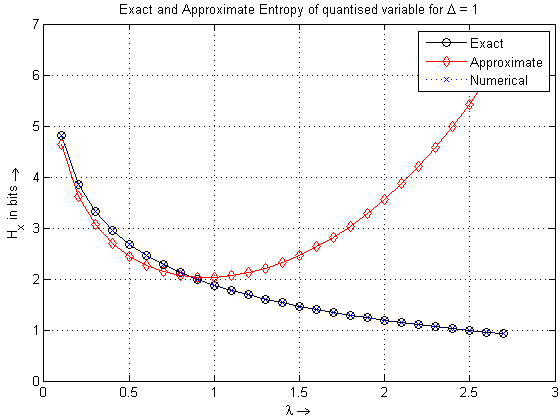
\includegraphics[width=0.95\textwidth,keepaspectratio]{003_001_approx1.png}
\end{figure}

\subsubsection{Exact Result}

The exact result, from the graph above, may be obtained by plugging in the exact values for $u_{1,2}(\lambda)$ into equation (\ref{eqn:hh}). The exact values may be computed starting from the following identities.

\begin{align} 1 &= \int_{0}^{\infty} \varphi(x) dx = \int_{0}^{\frac{\Delta}{2}} \varphi(x) dx + \sum_{\hat{x} \in \hat{X}} \int_{\hat{x} - \frac{\Delta}{2}}^{\hat{x} + \frac{\Delta}{2}} \varphi(x) dx \\ -h_x &= \int_{0}^{\infty} \varphi(x) \log \varphi(x) dx \nonumber \\ &= \int_{0}^{\frac{\Delta}{2}} \varphi(x) \log \varphi(x) dx + \sum_{\hat{x} \in \hat{X}} \int_{\hat{x} - \frac{\Delta}{2}}^{\hat{x} + \frac{\Delta}{2}} \varphi(x) \log \varphi(x) dx\end{align}

As the derivation is lengthy, we directly present the simplified result below.

\begin{align} u_1(\lambda) &= \frac{e^{-\lambda\frac{\Delta}{2}}}{e^{\lambda\frac{\Delta}{2}} - e^{-\lambda\frac{\Delta}{2}}} \\ u_2(\lambda) &= \frac{-h_x - c_1  - \frac{\Delta}{2}\lambda  \left[e^{\lambda\frac{\Delta}{2}} + e^{-\lambda\frac{\Delta}{2}}\right] u_1(\lambda)}{e^{\lambda\frac{\Delta}{2}} - e^{-\lambda\frac{\Delta}{2}}}\end{align}

Where $c_1 = log(\lambda) - 1 + \frac{\Delta}{2}\lambda e^{-\lambda\frac{\Delta}{2}}$. We see that even with a simple distribution function, the exact expressions quickly get out of hand and are unfortunately not short and elegant as one would have expected.

\subsubsection{Version History}
\begin{enumerate}
	\item \emph{First published: 3rd Oct. 2015 on aravindhk-math.blogspot.com}
	\item \emph{Modified: 16th Dec. 2023 -- Style updates for \LaTeX}
\end{enumerate}

\section{Entropy of Uniformly Quantized Laplace and Half-Laplace Distributions}

This post is about entropy of discrete stochastic variables that are derived by quantizing continuous stochastic variables. A good introduction to the concept of entropy in Information Theory is in [1]. This post is in continuation to the previous post in [2].

Let $x \in \mathbb{R}$ be a continuous stochastic variable with $\text{Laplace}(0, b)$ distribution and let $\hat{x} \in \hat{X}$ such that $\hat{X} \subset \mathbb{R}$ and $0 \in \hat{X}$ be its uniformly quantized version with step size $\Delta$. We would like to find the entropy of the discrete stochastic variable $\hat{x}$, denoted by $H_{\hat{x}}$, which provides us an estimate of the average number of bits required to encode $\hat{x}$.

HALF-LAPLACE DISTRIBUTION

Half-Laplace distribution refers to the distribution obtained by folding the zero-mean distribution function along the center. The new distribution is equivalent to the distribution of the stochastic variable $y = |x|$, i.e. the absolute value of the original Laplace distributed variable.

Let $\varphi(x)$ and $\Phi(x)$ denote the probability distribution function and cumulative distribution function of the Laplace variable $x$. These are defined as follows.

\begin{align}\varphi(x) &= \frac{1}{2b} e^{-\frac{|x|}{b}} \\ \Phi(x) &= \begin{cases} \frac{1}{2} e^{\frac{x}{b}} & \text{if $x < 0$} \\ 1 - \frac{1}{2} e^{-\frac{x}{b}} & \text{if $x \geq 0$}\end{cases}\end{align}

The half-Laplace cumulative distribution function of $y$, denoted by $\breve{\Phi}(y)$, is then given as follows.

\begin{align} \breve{\Phi}(y) &= \begin{cases} 0 & \text{if $y = 0$} \\ \Phi(y) - \Phi(-y) & \text{if $y > 0$}\end{cases} \\ &= 1 - e^{-\frac{y}{b}} \label{eqn:le} \end{align}

The expression in equation (\ref{eqn:le}) may be directly recognized as the cumulative distribution function of $\text{Exponential}(1/b)$. Therefore, the entropy of half-Laplace distribution may be found according to the expressions in [2] with $\lambda = 1/b$. 

LAPLACE DISTRIBUTION

Let $f(\hat{x})$ denote the probability mass function of the quantized variable $\hat{x}$. It is related to the probability density function $\varphi(x)$ as follows.
\begin{align} f(\hat{x}) = \int_{\hat{x} - \frac{\Delta}{2}}^{\hat{x} - \frac{\Delta}{2}} \varphi(x) dx \label{eqn:lq} \end{align}
Further, let $\hat{X}{}^+ \subset \hat{X}$ such that it contains the positive quantized values. The negative entropy $-H_{\hat{x}}$ is given (by definition) as follows. Note that the simplification is possible due to the symmetry of Laplace distribution.

\begin{align} -H_{\hat{x}} &= \sum_{\hat{x} \in \hat{X}} f(\hat{x}) \log f(\hat{x}) \\ &= f(0) \log f(0) + 2 \sum_{\hat{x} \in \hat{X}{}^+} f(\hat{x}) \log f(\hat{x}) \end{align}

By using the definition from equation (\ref{eqn:lq}) we have the following:

\begin{align} -H_{\hat{x}} &= \left(1 - e^{-\frac{\Delta}{2b}}\right) \log \left[1 - e^{-\frac{\Delta}{2b}} \right] \nonumber\\ &\quad +  \left(e^{\frac{\Delta}{2b}} - e^{-\frac{\Delta}{2b}}\right) \log \left[ \frac{1}{2} \left(e^{\frac{\Delta}{2b}} - e^{-\frac{\Delta}{2b}}\right) \right] v_1(b) \nonumber\\ &\quad + \left(e^{\frac{\Delta}{2b}} - e^{-\frac{\Delta}{2b}}\right) v_2(b) \end{align}

With the functions $v_{1,2}(b)$ given by:

\begin{align} v_1(b) &= \sum_{\hat{x} \in \hat{X}{}^+} e^{-\frac{\hat{x}}{b}} \\ v_2(b) &= \sum_{\hat{x} \in \hat{X}{}^+} e^{-\frac{\hat{x}}{b}} \log e^{-\frac{\hat{x}}{b}} \end{align}

EXACT RESULT

The analytical expressions for $v_{1,2}(b)$ may be computed starting from the following identities.

\begin{align} 1 &= \int_{-\infty}^{\infty} \varphi(x) dx = 2 \int_{0}^{\frac{\Delta}{2}} \varphi(x) dx + 2 \sum_{\hat{x} \in \hat{X}{}^+} \int_{\hat{x} - \frac{\Delta}{2}}^{\hat{x} + \frac{\Delta}{2}} \varphi(x) dx \\ -h_x &= \int_{-\infty}^{\infty} \varphi(x) \log \varphi(x) dx  \nonumber\\ &= 2 \int_{0}^{\frac{\Delta}{2}} \varphi(x) \log \varphi(x) dx + 2 \sum_{\hat{x} \in \hat{X}{}^+} \int_{\hat{x} - \frac{\Delta}{2}}^{\hat{x} + \frac{\Delta}{2}} \varphi(x) \log \varphi(x) dx \end{align}

Where $h_x$ is the differential entropy. Upon simplification, we obtain the following results.

\begin{align} v_1(b) &= \frac{e^{-\frac{\Delta}{2b}}}{e^{\frac{\Delta}{2b}} - e^{-\frac{\Delta}{2b}}} \\ v_2(b) &= \frac{-h_x - c_1 - \frac{\Delta}{2b} \left[ e^{\frac{\Delta}{2b}} + e^{-\frac{\Delta}{2b}} \right] v_1(b)}{e^{\frac{\Delta}{2b}} - e^{-\frac{\Delta}{2b}}}\end{align}

Where $c_1 = log\left(\frac{1}{2b}\right) - 1 + \frac{\Delta}{2b}e^{-\frac{\Delta}{2b}}$.

We see that the expressions are quite similar to the ones obtained for Exponential distribution in [2]. This is expected as Laplace and Exponential distributions are very closely related.

References:
[1] Thomas M. Cover, Joy A. Thomas, Elements of Information Theory, Second Edition, Wiley 2006.
[2] Aravindh Krishnamoorthy, Entropy of Uniformly Quantized Exponential Distribution, Applied Mathematics and Engineering Blog, October 2015.

\emph{First published: 5th Oct. 2015 on aravindhk-math.blogspot.com}

\section{Entropy of Sign-Magnitude Coding of Uniformly Quantized Laplacian Variables}

\emph{This is the third post in series discussing uniform quantization of Laplacian stochastic variables and is about entropy of separately coding sign and magnitude of uniformly quantized Laplacian variables.}

We begin by showing that the distribution of the magnitude of uniformly quantized Laplacian variable is the same as the distribution of uniformly quantized magnitude of the Laplacian variable which is shown in  Section \ref{sec:004_entropy} to be equivalent to the distribution of a corresponding uniformly quantized Exponential variable.

Let $\hat{x}$ be the uniformly quantized version, with step size $\Delta$, of a Laplacian variable $x$ with $\text{Laplace}(0,b)$ distribution and let $\hat{m}$ and $\hat{s}$ be the variables denoting magnitude and sign of $\hat{x}$ respectively. We have $\hat{m} = |\hat{x}| \in \{0, \mathbb{Z}^+\}$ and $\hat{s} = \text{sign}(\hat{x}) \in \{-1, 0, +1\}$.

Let $f_{\hat{x}}(\hat{x})$ and $\Phi_{\hat{x}}(\hat{x})$ denote the probability mass function and cumulative distribution function of $\hat{x}$ respectively. These are given as follows.

\begin{align}f_{\hat{x}}(\hat{x}) &= \begin{cases}1-e^{-\frac{\Delta}{2b}} & \text{if $\hat{x} = 0$}\\ \frac{1}{2}e^{-\frac{|\hat{x}|}{b}}\left(e^{\frac{\Delta}{2b}} - e^{-\frac{\Delta}{2b}}\right) & \text{otherwise}\end{cases}\\\Phi_{\hat{x}}(\hat{x}) &= \begin{cases}\frac{1}{2}e^{\frac{\hat{x}}{b}}e^{\frac{\Delta}{2b}} & \text{if $\hat{x} < 0$}\\1-\frac{1}{2}e^{\frac{\hat{x}}{b}}e^{-\frac{\Delta}{2b}} & \text{if $\hat{x} \geq 0$}\end{cases}\end{align}

The cumulative distribution function $\Phi_{\hat{m}}(\hat{m})$ of the discrete variable $\hat{m}$ is given as follows

\begin{align}\Phi_{\hat{m}}(\hat{m}) = \Phi_{\hat{x}}(\hat{m}) - \Phi_{\hat{x}}(-\hat{m}_{+1})\end{align},

where $\hat{m}_{+1} = \hat{m} + \Delta$ denotes the quantization point immediately succeeding $\hat{m}$. Substituting the value of $\Phi_{\hat{x}}(\hat{x})$ from above we have

\begin{align}\Phi_{\hat{m}}(\hat{m}) &= 1 - e^{-\frac{\hat{m}}{b}} e^{-\frac{\Delta}{2b}}\end{align},

which can be readily seen as the cumulative distribution function of a uniformly quantized Exponential variable $\text{Exponential}(1/b)$ quantized with step size $\Delta$. Therefore, the entropy of $\hat{m}$, denoted by $H_{\hat{m}}$, is as given in Section \ref{sec:003_entropy} . Note that a generic version of the above equivalence may be proven for distributions symmetric around zero.

Next, we find the entropy of the stochastic variable denoting the sign $\hat{s}$ which takes values from the set $\hat{S} = \{+1, 0, -1\}$. Let $f_{\hat{s}}(\hat{s})$ denote the probability mass function of the discrete variable $\hat{s}$. It is given as follows.

\begin{align}f_{\hat{s}}(\hat{s}) = \begin{cases}1 - e^{-\frac{\Delta}{2b}} & \text{if $\hat{s} = 0$}\\ \frac{1}{2} e^{-\frac{\Delta}{2b}} & \text{if $\hat{s} = \pm 1.$}\end{cases}\end{align}

Encoding $\hat{s} = 0$ carries no more information than what is contained in $\hat{m}$ as $\hat{s} = 0$ if and only if $\hat{m} = 0$. Therefore, we only need to encode the non-zero signs. The entropy of the reduced size alphabet may be computed using the theorem for general case given below.

Let $A = \{\chi_0, \chi_1, \cdots, \chi_n\}$ be a finite size coding alphabet with corresponding probabilities $P = \{p_0, p_1, \cdots, p_n\}$. Now let $D = \{d_0, d_1, \cdots, d_n\}$ be the probabilities that symbols from $A$ are coded. That is, if $d_i = 1$ then the i-th symbol is always coded, if $d_i = 0.5$ then it is coded 50\% of the times, and the other 50\% of the times it is inferred correctly at the decoder. There are no errors in the decoding process due to the reduced alphabet size. Let 
\begin{align}H_{A^{-}} = -\sum_{i = 1}^{n} p_i d_i \log \left( \frac{p_i d_i}{\sum_{j} p_j d_j} \right)\end{align}
denote the entropy of the reduced size coding alphabet. Then $H_{A^{-}}$ may be given by the straightforward result below.

For the case above for $\hat{s}$, we set $D = \{1, 0, 1\}$, that is, we would not encode the symbol '0' but infer it correctly based on the value of $\hat{m}$. We have entropy of coding $\hat{s}$ using this scheme, denoted by $H_{\hat{S}^-}$, given as follows.

\begin{align}H_{\hat{S}^-} &= -2\frac{1}{2} e^{-\frac{\Delta}{2b}} \log \frac{1}{2}\nonumber\\ &= e^{-\frac{\Delta}{2b}} \log 2\end{align}

Finally, using the values of entropy $H_{\hat{x}}$ and $H_{\hat{m}}$ from Sections \ref{sec:004_entropy} and \ref{sec:003_entropy} and $H_{\hat{S}^-}$ from above, we have the following upon simplification.

\begin{align}H_{\hat{x}} = H_{\hat{m}} + H_{\hat{S}^-}\end{align}

Therefore, encoding the magnitude and the reduced sign has the same entropy as encoding the uniformly quantized Laplacian variable.

\subsection{Version History}
\begin{enumerate}
	\item \emph{First published: 29th Oct. 2015 on aravindhk-math.blogspot.com}
	\item \emph{Modified: 17th Dec. 2023 -- Style updates for \LaTeX}
\end{enumerate}

\section{Exact Formula for Asymptotic Convergence of Fourier Transform of Uniform Random Variables}

It is well known that the distribution of sums of random variables converges to Gaussian. In this post, we look look at the convergence of Fourier transform of uniformly distributed random variables.

Exact and analytical formulas for convergence are interesting as they help develop an intuition about the asymptotic convergence phenomenon and understand the convergence error for finite number  of samples. Under the scanner today is the convergence behaviour of Fourier transform of uniformly distributed random variables (URVs). 

Let $u_1, u_2, \cdots, u_N$ denote complex-valued zero mean i.i.d URVs with finite support $[-q_n, q_n]\times [-q_n, q_n]$ for $n = 1\cdots N$. Their Fourier transform is given by
\begin{align}U_k = \frac{1}{\sqrt{N}} \sum_{n = 1}^{N} u_n W^{kn} = \frac{1}{\sqrt{N}} \sum_{n = 1}^{N} v_n,\end{align}
where $W^{kn}$ are the roots of unity, and $v_n = u_n W^{kn}$.

Let $U^r_k = \mathfrak{Re}(U_k)$, and $v^r_n = \mathfrak{Re}(v_n)$. Variable $v^r_n$ preserves the distribution of $\mathfrak{Re}(u_n)$. Therefore, we have the characteristic function of the real part of the Fourier transformed variable as
\begin{align}\text{E}(e^{itU_k^r}) &= \prod_{n = 1}^{N} \text{E}(e^{\frac{1}{\sqrt{N}}it v^r_n})\nonumber \\ &= \prod_{n = 1}^{N} \int_{-q_n}^{q_n} \frac{1}{2q_n} e^{\frac{1}{\sqrt{N}}it v^r_n} dv^r_n \nonumber\\ &= \prod_{n = 1}^{N} \frac{e^{\frac{1}{\sqrt{N}}itq_n} - e^{-\frac{1}{\sqrt{N}}itq_n}}{\frac{2}{\sqrt{N}}itq_n} \nonumber\\ &= \exp\left( \sum_{n = 1}^{N} \log \frac{\sin\left(\frac{1}{\sqrt{N}}tq_n\right)}{\frac{1}{\sqrt{N}}tq_n}\right).\end{align}

Interestingly, for $f(t) = \log \frac{\sin(t\alpha)}{t\alpha}$, the limits of the derivatives $\lim_{t\to 0} \frac{\text{d}^n f(t)}{\text{d}t^n}$, for $n = 1, 2, \cdots$, exist! Therefore, the Taylor expansion of $f(t)$ around $t=0$ is given by
\begin{align}f(t) = -\frac{t^2\alpha^2}{6} - \frac{t^4\alpha^4}{180} - \frac{t^6\alpha^6}{2835} + \cdots.\end{align}
The Taylor series expansion given above may be easily verified using symbolic solvers like Wolfram Alpha Online.

Substituting the Taylor series expansion in the characteristic function above, we have (only the first two terms of the Taylor series are shown)
\begin{align}\text{E}(e^{itU_k^r}) = \exp\left(-\frac{1}{6} \frac{t^2 \sum_{n = 1}^{N} q^2_n}{N} - \frac{1}{180}\frac{t^4 \sum_{n = 1}^{N} q^4_n}{N^2} + \cdots\right). \label{eqn:cg}\end{align}

Therefore, as $N\to \infty$, 
\begin{align}\lim_{N\to \infty} \text{E}(e^{itU_k^r}) = \exp\left(-\frac{t^2}{2} \frac{\bar{q}^2}{3}\right), \label{eqn:acg} \end{align}
where
\begin{align}\bar{q}^2 = \lim_{N\to \infty} \frac{1}{N}\sum_{n = 1}^{N} q_n^2.\end{align}

The right hand side expression in (\ref{eqn:acg}) showing the asymptotic convergence of the characteristic function of $U^r_k$ is readily identified as the characteristic function of Gaussian distribution with zero mean and variance $\bar{q}^2/3$. A similar expression may also be found for $\lim_{N\to \infty} \text{E}(e^{itU_k^i})$ in a straightforward manner.

Therefore, the exact convergence formula for the Fourier transform of URVs is as shown in (\ref{eqn:cg})!

ARK

\emph{First published: 25th Jun. 2016 on aravindhk-math.blogspot.com}

\section{Generating and Sampling Two Signed Bernoulli Random Variables with Given Correlation}

The following first constructs two signed $\{-1, +1\}$ Bernoulli variables $Y_1, Y_2$ such that $p(Y_1 = -1) = p_1, p(Y_2 = -1) = p2,$ and $E[Y_1Y_2] = r.$ Constraints: $0 < p1, p2 < 1, -1 < r < 1.$ 

Next, it draws $N$ realizations of the two variables in $Y(m,:), m = 1,2.$ The sample pdf and cross correlation converge as $N \to \infty.$

\subsection{MATLAB Reference Code}

To generate $N$ realizations of variables with mean $0,$ variance $1,$ and correlation $0.3$ using the code below, use: \texttt{Y = signed\_bernoulli2(N,0.5,0.5,0.3)}.

\begin{lstlisting}[language=MATLAB,numbers=none]
function Y = signed_bernoulli2(N,p1,p2,r)
% Y = signed_bernoulli2(N,p1,p2,r) 
% The function first constructs two(2) signed {-1, +1} Bernoulli variables
% Y_1, Y_2 such that p(Y_1 = -1) = p1, p(Y_2 = -1) = p2, and E[Y_1Y_2] = r.
% Constraints: 0 < p1,p2 < 1, -1 < r < 1.
% Next, it draws N realizations of the two variables in Y(m,:), m = 1,2.
% The sample pdf and cross correlation converge as N -> infinity (obviously).
%
% Example: generate N realizations of variables with mean 0, variance 1, and
% correlation 0.3: Y = signed_bernoulli2(N,0.5,0.5,0.3).
%
% Author: aravindh.krishnamoorthy@fau.de, on: 26.10.2017.

% Basic checks and initialization
assert (0 < p1) ;
assert (p1 < 1) ;
assert (0 < p2) ;
assert (p2 < 1) ;
assert (-1 < r) ;
assert (r < 1) ;
Y = zeros(2,N) ;

% Resolve the joint pdf given by
%                /  p(1) if (+1, +1)
% p(Y_1, Y_2) =  |  p(2) if (+1, -1)
%                |  p(3) if (-1, +1)
%                \  p(4) if (-1, -1)
%
% Conditions (i.e. how matrices A and b are generated):
% row 1: p(1) + p(2) + p(3) + p(4) = 1
% row 2: p(3) + p(4) = p1   -> marginal for Y_1
% row 3: p(2) + p(4) = p2   -> marginal for Y_2
% row 4: p(1) - p(2) - p(3) + p(4) = r   -> cross correlation E[Y_1 Y_2]

A = [1,1,1,1;0,0,1,1;0,1,0,1;1,-1,-1,1] ;
b = [1;p1;p2;r] ;
p = pinv(A)*b ;
assert(all(p >= 0), sprintf('The given p1=%f and p2=%f cannot result in a correlation r=%f with the given algorithm.\np1=p2=0.5 is a safe value.',p1,p2,r)) ;

% Now that we have the joint pdf in "p" we can draw from this distribution
% as follows (based on conditional pdfs and inverse transform sampling):
% 1. Draw samples of Y_1 from Signed_Bernoulli(p1) in a standard fashion using
%    an auxiliary uniformly distributed variable U_1 = U(1,:).
% 2. If the n-th sample of Y_1 is "-1", then draw for Y_2 from the conditional pdf
%    p(Y_2|Y_1 = -1) using a second axiliary uniformly distributed
%    variable U_2 = U(2,:).
% 2. If the n-th sample of Y_1 is "+1", then draw for Y_2 from the conditional pdf
%    p(Y_2|Y_1 = +1) using the second axiliary uniformly distributed
%    variable U_2 = U(2,:).
% The conditional pdfs are given as follows:
% p(Y_2|Y_1 = -1) = p(4)/p1 for -1, and 1-(p(4)/p1) for +1.
% p(Y_2|Y_1 = +1) = p(2)/(1-p1) for -1, and 1-(p(2)/(1-p1)) for +1.
%
% Note: for the rather straightforward proofs for the above steps, please contact
% the author.

% Auxiliary variable U
U = rand(2,N) ;

% Draw samples from p(Y_1)
Y(1,:) = (-1).^(U(1,:) < p1) ;

% Indices to help choose the conditional pdf
I1 = Y(1,:) == -1 ;
I2 = Y(1,:) == +1 ;

% Draw samples from the conditional pdfs
Y(2,I1) = (-1).^(U(2,I1) < p(4)/p1) ;
Y(2,I2) = (-1).^(U(2,I2) < p(2)/(1-p1)) ;
\end{lstlisting}

The full program can be downloaded at: \href{https://www.mathworks.com/matlabcentral/fileexchange/65164-signed_bernoulli2-n-p1-p2-r}{signed\_bernoulli2(N,p1,p2,r) - File Exchange - MATLAB Central (mathworks.com)}.

\subsection{Version History}
\begin{enumerate}
	\item \emph{First published: 23rd Nov. 2017 on aravindhk-math.blogspot.com}
	\item \emph{Modified: 17th Dec. 2023 -- Style updates for \LaTeX}
\end{enumerate}


\section{Distribution of A Simple Function of Gamma Variables}

In this post, we look at a nifty result presented in [Krishnamoorthy2019] where the probability density function (pdf) of the function $\dfrac{r_1}{c+r_2}$ two independent Gamma distributed random variables $r_1 \sim \mathcal{G}(k_1,\theta_1)$ and $r_2 \sim \mathcal{G}(k_2, \theta_2)$ is derived.

The derivation is an exercise (for the scalar case) in computing the pdf of functions of variables by constructing the joint pdf and marginalizing based on the Jacobian. A similar approach can also be used for matrix-variate distributions (which will probably be a good topic for another post.)

Theorem

Let $c > 0,$ and let $r_1 \sim \mathcal{G}(k_1,\theta_1)$ and $r_2 \sim \mathcal{G}(k_2, \theta_2)$ be independent random variables, then, the pdf of $r = \dfrac{r_1}{c+r_2}$, denoted by $p_r(r;k_1,\theta_1,k_2,\theta_2,c),$ is given by

\begin{equation}K_\mathrm{r} r^{k_1-1} \exp\left(-\frac{rc}{\theta_1}\right) U\left(k_2,k_1+k_2+1;c\left(\frac{r}{\theta_1}+\frac{1}{\theta_2}\right)\right),\end{equation}

where $$U(a,b;z) = \frac{1}{\Gamma(a)} \int_{0}^{+\infty} \exp(-zx) x^{a-1} (1+x)^{b-a-1} \mathrm{d}x$$ is the hypergeometric U-function [Olver2010, Chapter 13, Kummer function], and $K_\mathrm{r}$ is a constant ensuring that the integral over the pdf equals one.

Proof

As $r_1$ and $r_2$ are independent, their joint pdf, denoted by $p_{r_1,r_2}(r_1,r_2;k_1,\theta_1,k_2,\theta_2),$ is given by

\begin{equation}\frac{1}{\Gamma(k_1) \theta_1^{k_1} \Gamma(k_2) \theta_2^{k_2}} r_1^{k_1-1} r_2^{k_2-1} \exp\left(-\frac{r_1}{\theta_1}-\frac{r_2}{\theta_2}\right).\end{equation}

Applying transformation $r = \frac{r_1}{c+r_2}$ with Jacobian $\frac{\mathrm{d} r_1}{\mathrm{d} r} = c+r_2,$ we obtain the transformed pdf, $p_{r,r_2}(r,r_2;k_1,\theta_1,k_2,\theta_2,c)$, as

\begin{align}K_\mathrm{r}' r^{k_1-1} (c+r_2)^{k_1} r_2^{k_2-1}\exp\left(-\frac{rc}{\theta_1}-\left(\frac{r}{\theta_1} +\frac{1}{\theta_2}\right)r_2\right),\end{align}

where $K_\mathrm{r}'$ is a constant ensuring that the integral over the pdf equals one. Next, 
$p_r(r;k_1,\theta_1,k_2,\theta_2,c)$ is obtained by marginalization as

\begin{equation}p_r(r;k_1,\theta_1,k_2,\theta_2,c) = \int_{0}^{+\infty} \hspace{-0.25cm} p_{r,r_2}(r,r_2;k_1,\theta_1,k_2,\theta_2,c) \mathrm{d} r_2,\end{equation}

where the integration is conducted using the integral representation of the hypergeometric U-function from [Olver2010, Chapter 13, Kummer function] to obtain the expression in the theorem statement.

References

[Krishnamoorthy2019] A. Krishnamoorthy and R. Schober, “Precoder design for two-user uplink MIMO-NOMA with simultaneous triangularization,” in Proc. IEEE Global Commun. Conf., Dec. 2019, pp. 1–6. https://doi.org/10.1109/GLOBECOM38437.2019.9014161
[Olver2010] F. W. Olver, D. Lozier, R. Boisvert and C. Clark, "NIST digital library of mathematical functions", Release, vol. 1, pp. 14, 2010.

\emph{First published: 19th Oct. 2021 on aravindhk-math.blogspot.com}

\subsection{Distribution of the Determinant of a Complex-Valued Sample Correlation Matrix}

\emph{In this post, we look at the distribution of the determinant of the sample correlation matrix of the realizations of a complex-valued Gaussian random vector. The distribution for real-valued Gaussian random vector was developed in \cite{PhamGia2014}, and we largely follow the developed framework. Thanks to Prashant Karunakaran for bringing this problem and the many applications to my attention in late 2017/early 2018.}

Let $\boldsymbol{x}$ be a Gaussian random vector of length $p$ with mean $\boldsymbol{\mu} \in \mathbb{C}^p$ and covariance $\boldsymbol{\Sigma} \in \mathbb{C}^{p\times p}.$ Let $\boldsymbol{x}^{(1)}, \boldsymbol{x}^{(2)}, \dots, \boldsymbol{x}^{(n)}$ denote $n$ realizations, $n \geq p,$ of $\boldsymbol{x}.$ In the terminology of \cite{PhamGia2014}, the adjusted sample covariance matrix is given by $$\boldsymbol{S} = \frac{1}{n}\sum_{i = 1}^{n}(\boldsymbol{x}^{(i)} - \bar{\boldsymbol{x}})(\boldsymbol{x}^{(i)} - \bar{\boldsymbol{x}})^\mathrm{H},$$ where $\bar{\boldsymbol{x}}$ is the sample mean given by $$\bar{\boldsymbol{x}} = \frac{1}{n}\sum_{i = 1}^{n}\boldsymbol{x}^{(i)}.$$ Note that the adjusted sample covariance matrix is positive semi-definite.

The correlation matrix $\boldsymbol{R}$ is defined as: $$\boldsymbol{R} = \boldsymbol{D}^{-\frac{1}{2}} \boldsymbol{S} \boldsymbol{D}^{-\frac{1}{2}},$$ where $\boldsymbol{D} = \mathrm{Diag}(\boldsymbol{S})$ is a diagonal matrix with the diagonal elements of $\boldsymbol{S}$ on the main diagonal. Hence, $\boldsymbol{R}$ has unit diagonal elements and is independent of the variance of the elements of $\boldsymbol{x}.$ 

Now, for real-valued $\boldsymbol{x},$ the determinant of $\boldsymbol{R},$ denoted by $|\boldsymbol{R}|,$ is shown in \cite[Theorem 2]{PhamGia2014} to be a product of $p-1$ Beta-distributed scalar variables $\mathrm{Beta}(\frac{n-i}{2},\frac{i-1}{2}),$  $i=1,\dots,p-1.$ The density of the product can be given in terms of the \href{https://mathworld.wolfram.com/MeijerG-Function.html}{$\mathrm{MeijerG}$ function} as follows \cite[Theorem 2]{PhamGia2014}:

$$g_\mathbb{R}(x;n,p) = \frac{\left[\Gamma(\frac{n-1}{2})\right]^{(p-1)} }{\Gamma(\frac{n-2}{2})\dots\Gamma(\frac{n-p}{2})} \mathrm{MeijerG}^{\begin{bmatrix}p-1 & 0 \\ p-1 & p-1\end{bmatrix}}\left(x\middle|\begin{matrix}\frac{n-3}{2},\dots,\frac{n-3}{2}\\ \frac{n-4}{2},\dots,\frac{n-(p+2)}{2}\end{matrix}\right).$$

Analogously, for complex-valued $\boldsymbol{x},$ $|\boldsymbol{R}|$ is a product of $p-1$ Beta-distributed scalar variables $\mathrm{Beta}(n-i,i),$  $i=1,\dots,p-1.$ The density of the product can now be given in terms of the $\mathrm{MeijerG}$ function, in a straightforward manner, as follows.

$$g_\mathbb{C}(x;n,p) = \frac{\left[\Gamma(n-1)\right]^{(p-1)} }{\Gamma(n-1)\dots\Gamma(n-p+1)} \mathrm{MeijerG}^{\begin{bmatrix}p-1 & 0 \\ p-1 & p-1\end{bmatrix}}\left(x\middle|\begin{matrix}n-1,\dots,n-1\\ n-2,\dots,n-p\end{matrix}\right).$$

In the following, a Mathematica program for numerical simulation and the corresponding output are provided.

\begin{lstlisting}[language=Mathematica,numbers=none]
gC[x_, n_,p_] := (Gamma[n])^(p - 1) / 
	Product[Gamma[n - i], {i, 1, p - 1}] MeijerG[{{},
	Table[n - 1, {i, 1, p - 1}]}, {Table[n - i, {i, 2, p}], {}}, x]

r[x_] := Module[{d}, d = DiagonalMatrix[Diagonal[x]]; 
MatrixPower[d, -1/2] . x . MatrixPower[d, -1/2]]

\[ScriptCapitalD] =
MatrixPropertyDistribution[Det[r[(xr + I xi) .
ConjugateTranspose[xr + I xi]]], {xr \[Distributed]
	MatrixNormalDistribution[IdentityMatrix[p], IdentityMatrix[n]],
	xi \[Distributed]
	MatrixNormalDistribution[IdentityMatrix[p],
	IdentityMatrix[n]]}] ;

data = Re[RandomVariate[\[ScriptCapitalD], 100000]] ;
\[ScriptCapitalD]1 = SmoothKernelDistribution[data] ;

Plot[{PDF[\[ScriptCapitalD]1, x], gC[x, n, p]}, {x, 0, 1},
	PlotLabels -> {"Numerical", "Analytical"},
	AxesLabel -> {"u", "p(u)"}]
\end{lstlisting}

The following figure shows that the numerical and analytical results match perfectly for the example case $n=4, k=6.$

\begin{figure}[H]
	\centering
	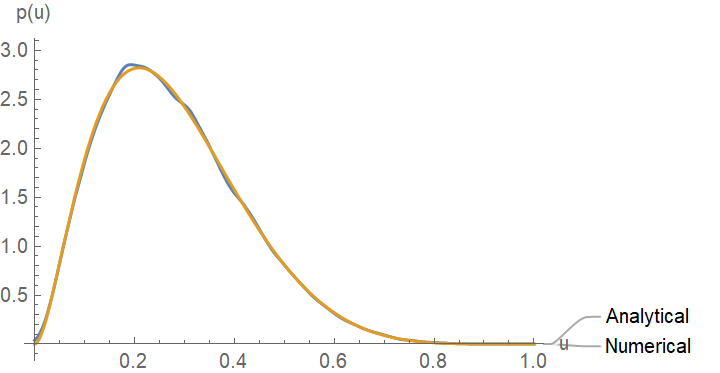
\includegraphics[width=0.95\textwidth,keepaspectratio]{014_001_Fig_Det_R.png}
\end{figure}

\subsubsection{Version History}
\begin{enumerate}
	\item \emph{First published: 12th Dec. 2021 on aravindhk-math.blogspot.com}
	\item \emph{Modified: 17th Dec. 2023 -- Style updates for \LaTeX}
\end{enumerate}


\chapter{Random Matrix Theory}
\subsection{Stochastic Properties of Random Matrix Factors - 1}

\emph{In this series of posts, we will be considering the stochastic properties of factors of random matrices. At first, we look at the simple case of Cholesky decomposition of \href{https://en.wikipedia.org/wiki/Wishart_distribution}{Wishart matrices}. More below.}

Let $H$ be a matrix whose elements are random variables, each with a given distribution. Now assume that we factorize $H$ using one of the matrix factorization techniques such as QR, Eigenvalue, or Cholesky decomposition. The elements of the matrix factor are also random variables... but what are their distributions?

This is exactly what we hope to answer.

First and the obvious reason to find the distributions is to understand the characteristics of the matrix factor. For example, in a wireless communication MIMO channel, which is a zero-mean Gaussian random matrix, it helps us understand the stochastic properties of a "partial" or "inverse" channel.

The second reason is to speed up simulations. If we have a simulation that requires a random matrix factor which is computed numerically, the simulation may be sped up by generating the elements of the matrix factor directly with the given distributions.

Now we look at the stochastic properties of Cholesky decomposition of Wishart matrices.

Let $G \in \mathbb{C}^{n \times n}$ be a complex-valued matrix whose elements are Gaussian random variables i.e. $\mathcal{N}(0,1)$. Let $H = G^H G$. $H$ (Wishart matrix) is now a Hermitian symmetric complex-valued matrix.

It is well known that the Cholesky decomposition of $H$ is the upper triangular matrix from the QR decomposition of $G$, i.e. $H = R^H R$ where $G = QR$ for a Unitary matrix $Q$ and an upper triangular matrix with positive diagonal elements $R$.

Therefore, the distribution of $R$ is straightforward from \cite{Edelman2005} and is given as follows:
$$
\begin{bmatrix}
	\chi_n & \mathcal{N} & \cdots & \mathcal{N} \\
	& \chi_{n-1} & \cdots & \mathcal{N} \\
	&                   & \ddots & \vdots \\
	&                   &            & \chi_1
\end{bmatrix},
$$

where $\mathcal{N}$ denotes Gaussian distribution and $\chi_k$ the Chi distribution with $k$ degrees of freedom.

Stochastic properties of the matrix factors may also be verified numerically. Let $G \in \mathbb{R}^{2 \times 2}$ be a real-valued matrix with elements distributed according to standard Gaussian distribution, i.e. $g_{ij}$'s are $\mathcal{N}(0,1)$. $G \leadsto R$ given by:
$$
\begin{bmatrix}
	\mathcal{N}(0,1) & \mathcal{N}(0,1) \\
	\mathcal{N}(0,1) & \mathcal{N}(0,1)
\end{bmatrix} \leadsto
\begin{bmatrix}
	\chi_2 & \mathcal{N}(0,1) \\
	& \chi_1
\end{bmatrix}
$$

Figure below illustrates the distributions of elements of $R$ computed numerically using MATLAB. Normalized numerical quantities obtained over 100000 trials are plotted in the blue bar graph and the theoretical expectation is plotted in red. Numerical results closely match the theoretical expectation.

\begin{figure}[H]
	\centering
	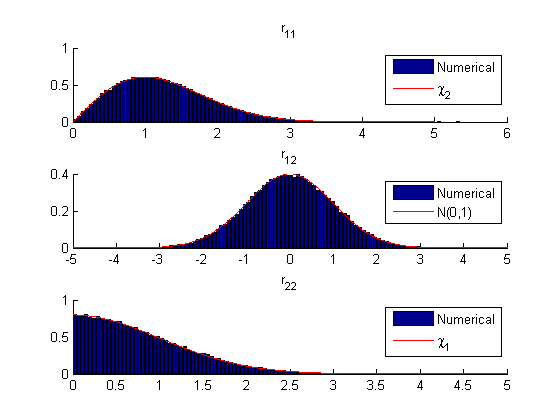
\includegraphics[width=0.95\textwidth,keepaspectratio]{002_001_mfs1.png}
	\caption{Numerical vs theoretical distribution of elements of R.}
\end{figure}

In the next blog posts on this topic, I hope to be able to provide more examples for stochastic properties of matrix factors especially the ones we come across in wireless communication.

\subsubsection{Version History}
\begin{enumerate}
	\item \emph{First published: 22nd Sep. 2015 on aravindhk-math.blogspot.com}
	\item \emph{Modified: 17th Dec. 2023 -- Style updates for \LaTeX}
\end{enumerate}

\subsection{Stochastic Properties of Random Matrix Factors - 2}

In the second on the series of posts on stochastic properties of factors of random matrices, we look at a yet another simple case involving norm square of elements of QR decomposition of a scaled Rayleigh matrices. More below.

In applications such as Non-Orthogonal Multiple Access (NOMA), the so-called "path loss" plays an important role whereby a channel matrix $\mathbf{H}$ at a receiver is better modelled as a scaled Rayleigh matrix given by $$\mathbf{H} = \frac{1}{\sqrt{L}} \mathbf{G}$$ where $L > 0$ is the path-loss factor and $\mathbf{G}$ the conventional Rayleigh matrix with real and imaginary parts of the elements each $\mathcal{N}(0,1)$.

Let (by QR decomposition) $\mathbf{H} = \mathbf{Q}\mathbf{R}$ where $\mathbf{Q} \in \mathbb{C}^{M\times M}$ is a Unitary matrix, and $\mathbf{R} \in \mathbb{C}^{M\times N}$ is upper triangular. The distribution of the norm square of elements, $|[\mathbf{R}]_{ij}|^2$, of $\mathbf{R}$ is given by $$|[\mathbf{R}]_{ij}|^2 \sim \begin{cases} \Gamma(M+1-i,\frac{2}{L}) & \text{if $i = j$} \\ \Gamma(1,\frac{2}{L}) & \text{if $i < j$} \\ 0 & \text{otherwise,} \end{cases}$$ where $i=1,2,\cdots,M$, $j=1,2,\cdots,N$, and $\Gamma(k,\theta)$ denotes the Gamma distribution with probability density function $$f(x; k,\theta) = \frac{1}{\Gamma(k)\theta^k}x^{(k-1)}e^{-\frac{x}{\theta}}$$ where $\Gamma(k)$ is the complete Gamma function.

The stochastic properties of the diagonal elements of $\mathbf{R}$ are interesting as they can be used to derive insights, amongst others, about mutual information of "layers" (i.e. parallel streams of information, one per row) or the determinant of the covariance matrix of $\mathbf{H}$.

Figure below illustrates the distributions of elements of $\mathbf{R}$ for $M=4, N=2$ computed numerically using MATLAB. Normalized numerical quantities obtained over 100000 trials are plotted in the blue bar graph and the theoretical expectation is plotted in red. Numerical results closely match the theoretical expectation.

\begin{figure}[H]
	\centering
	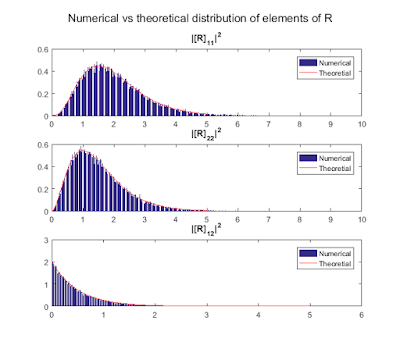
\includegraphics[width=0.95\textwidth,keepaspectratio]{008_001_smf-2.png}
\end{figure}

ARK

\subsubsection{Version History}
\begin{enumerate}
	\item \emph{First published: 25th Aug. 2017 on aravindhk-math.blogspot.com}
	\item \emph{Modified: 17th Dec. 2023 -- Style updates for \LaTeX}
\end{enumerate}

\section{Stochastic Properties of Random Matrix Factors - 3}

In this third post continuing QR and related Cholesky matrix decomposition techniques, we look at the probability density function (PDF) of a diagonal element of the QR decomposition of a complex-valued random matrix with circular Gaussian i.i.d elements.

Let $\mathbf{H}$ denote an $N\times N$ matrix with circular Gaussian independent and identically distributed (i.i.d) elements with zero mean and variance two i.e. $\mathcal{CN}(0,2)$. Furthermore let $\mathbf{R}$ denote the upper-triangular matrix obtained after QR decomposition ($\mathbf{H} = \mathbf{Q}\mathbf{R}$) such that the diagonal elements of $\mathbf{R}$ are non-negative. It is well-known that such a QR decomposition (QRP or QR with positive diagonal elements) of a matrix is unique. In case a QR decomposition algorithm results in negative diagonal elements, non-negativity may be arranged by multiplying those rows of $\mathbf{R}$ and the corresponding columns of $\mathbf{Q}$ by -1.

It is well known that the diagonal elements of $\mathbf{R}$ follow the distribution:
$$
\begin{bmatrix}
	\chi_{2N} & \mathcal{CN}(0,2) & \cdots &  \mathcal{CN}(0,2)\\
	& \chi_{2(N-1)} & \ddots & \vdots\\
	& & \ddots & \mathcal{CN}(0,2)\\
	& & & \chi_{2}
\end{bmatrix},
$$
where $\chi_{k}$ denotes a Chi-distributed random variable with $k$ degrees of freedom.

From the above, it follows that the distribution of a diagonal element $r$ of the matrix $\mathbf{R}$ may be given as the (equal) weighted sum of the pdfs of the diagonal elements as
$$
f_r(x) = \frac{1}{N} \sum_{n=1}^{N} \frac{2^{n}}{\Gamma(n)} x^{n-1} e^{-\frac{x}{2}},
$$
where $\Gamma(n)$ is the Gamma function.

The following graph shows the results of a MATLAB simulation for $N=4$ over 100000 iterations where the diagonal values of $\mathbf{R}$ were collected. The blue graph shows the histogram of the diagonal values. The red graph shows the pdf as obtained using the equation above. We notice that the two correspond well.

\begin{figure}[H]
	\centering
	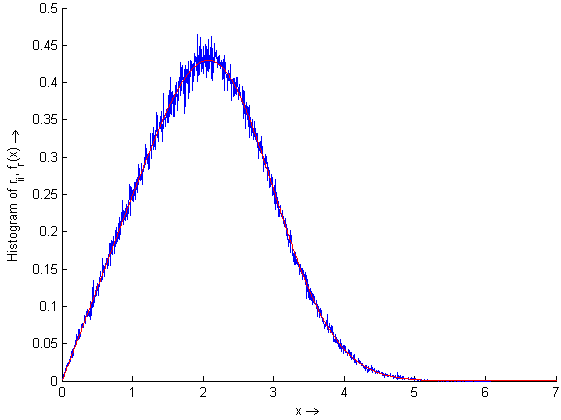
\includegraphics[width=0.95\textwidth,keepaspectratio]{010_001_frx.png}
\end{figure}

ARK

\subsection{Version History}
\begin{enumerate}
	\item \emph{First published: 29th Dec. 2017 on aravindhk-math.blogspot.com}
	\item \emph{Modified: 17th Dec. 2023 -- Style updates for \LaTeX}
\end{enumerate}

\section{Ordered densities of squared singular values of a Gaussian matrix product}

%%%%%%%%%%%%%%%%%%%%%%%%%%%%%%%%%%%%%%%%%%%%%%%%%%%%%%%%%%%%%%%%%%%%%%%%%%%%%%%%
% 015 Math macros
\newcommand{\G}[7]{\mathrm{G}^{\tiny\begin{bmatrix}
			#1&#2\\#3&#4
	\end{bmatrix}}\left(\begin{matrix}
		#5 \\ #6
	\end{matrix}\;\middle|\;#7\right)}
%%%%%%%%%%%%%%%%%%%%%%%%%%%%%%%%%%%%%%%%%%%%%%%%%%%%%%%%%%%%%%%%%%%%%%%%%%%%%%%%

This rather simple result is a humble acknowledgement of the great work in finite-size random matrix theory (RMT) by Prof. Gernot Akemann and team at Uni Bielefeld. For finding the ordered densities, a straightforward recursive formulation, in terms of the MeijerG function, based on the work of Alberto Zanella at CNR in Italy, is utilized.

Note: Several integration formulas for the MeijerG function are known, e.g., see the MeijerG function reference.
Although the expressions are complex, they can be numerically evaluated quite easily via Mathematica or MATLAB. It amazes me that these finite-size RMT densities are even analytically approachable, although, undoubtedly, the asymptotic RMT theory is "more elegant."

The theorem is as follows. See below for Mathematica code and numerical simulations.

Theorem

\begin{theorem}
	\label{thm:qk}
	Let $\boldsymbol{X}$ and $\boldsymbol{Y}$ be independent $m\times l$ and $l\times q$ random matrices, respectively, $q \leq m \leq l,$ with identical and independently distributed elements $[\boldsymbol{X}]_{ij}, \sim \mathcal{CN}(0,1), i=1,\dots,m,j=1,\dots,l,$ and $[\boldsymbol{Y}]_{ij}, \sim \mathcal{CN}(0,1), i=1,\dots,l,j=1,\dots,q,$ respectively. Let $x_1 \geq \dots \geq x_q$ denote the squared singular values of the product $\boldsymbol{X}\boldsymbol{Y}.$ The pdf of the $k$-th squared singular value of $\boldsymbol{X}\boldsymbol{Y},$ denoted by $q_k(x_k; m, l, q),$ is given by
	\begin{align}
		q_k(x_k; m, q) = K_{q_k} h^{[k,(),()]}_k(x_k; m, l, q),
	\end{align}
	where $K_{q_k}$ is a constant ensuring that the integral over the pdf is equal to one, and function $h^{[d,\boldsymbol{n},\boldsymbol{m}]}_k(x_k; m, q)$ is given by the recurrence relation
	\begin{align}
		\sum_{i = 1}^{|{\mathcal{I}}^{[d,\boldsymbol{n}]}|} \sum_{j = 1}^{|{\mathcal{I}}^{[d,\boldsymbol{m}]}|} h^{[d-1,\boldsymbol{n}',\boldsymbol{m}']}_k(x_k; m,l,q), \label{eqn:qkrec}
	\end{align}
	$[l,(),()]$ denotes the initial value of $[d,\boldsymbol{n},\boldsymbol{m}],$ and ``()'' denotes the empty tuple. Tuples $\boldsymbol{n}$ and $\boldsymbol{m}$ are updated as $\boldsymbol{n}' \coloneqq \boldsymbol{n} \cup \{(i,[{\mathcal{I}}^{[d,\boldsymbol{n}]}]_i)\}$ and $\boldsymbol{m}' \coloneqq \boldsymbol{m} \cup \{(j,[{\mathcal{I}}^{[d,\boldsymbol{m}]}]_j)\},$ where $i$ and $j$ are the summation indices in (\ref{eqn:qkrec}), and $[{\mathcal{I}}^{[d,\boldsymbol{n}]}]_i$ and $[{\mathcal{I}}^{[d,\boldsymbol{m}]}]_j$ are the $i$-th and $j$-th elements of sets ${\mathcal{I}}^{[d, \boldsymbol{n}]}$ and ${\mathcal{I}}^{[d, \boldsymbol{m}]},$ respectively, defined as ${\mathcal{I}}^{[d,\boldsymbol{n}]} \coloneqq \{1,2,\dots,q\} \setminus \pi_2(\boldsymbol{n})$ and ${\mathcal{I}}^{[d,\boldsymbol{m}]} \coloneqq \{1,2,\dots,q\} \setminus \pi_2(\boldsymbol{m}).$ Next, the termination step is given in (\ref{eqn:qkf2term}) on top of this page,
	\begin{figure*}
		\begin{align}
			h^{[1,\boldsymbol{n},\boldsymbol{m}]}_k(x_k; m, q) &= \sum_{i = 1}^{|{\mathcal{I}}^{[d,\boldsymbol{n}]}|} \sum_{j = 1}^{|{\mathcal{I}}^{[d,\boldsymbol{m}]}|} s\left(\boldsymbol{n}',\boldsymbol{m}'\right)
			\G{2}{0}{0}{2}{-}{v_2+n-1, m+n+v_1-2}{x_k} \nonumber\\
			&\qquad \times \det{\boldsymbol{\Xi}\left(k, m, q, {\mathcal{I}}^{[d+1,\boldsymbol{n}']},{\mathcal{I}}^{[d+1,\boldsymbol{m}']}\right)} \nonumber\\
			&\qquad \times \prod_{p = 1}^{k-1} \G{3}{0}{1}{3}{1}{0, v_2+[{\mathcal{I}}^{[d,\boldsymbol{n}]}]_p, [{\mathcal{I}}^{[d,\boldsymbol{m}]}]_p + [{\mathcal{I}}^{[d,\boldsymbol{n}]}]_p+v_1 - 1}{x_k}\label{eqn:qkf2term}
		\end{align}
		\hrulefill
	\end{figure*}
	where $v_1=l-q, v_2=m-q,$ $G$ is the Meijer G function \cite{Olver2010}, $\boldsymbol{\Xi}\left(k, m, q, {\mathcal{I}}^{[d+1,\boldsymbol{n}']},{\mathcal{I}}^{[d+1,\boldsymbol{m}']}\right)$ is a $(q-l)\times (q-l)$ matrix with elements 
	\begin{equation}
		\left[\G{2}{1}{1}{3}{1}{v_2+n,m+n+v_1-1,0}{x_k}\right]_{ij}, \label{eqn:qkf2mat}
	\end{equation}
	and $i,j=1,\dots,q-l,$
	\begin{align}
		s\left(\boldsymbol{n}',\boldsymbol{m}'\right) &= (-1)^{\sum_{i=1}^{|\boldsymbol{n}'|} [\pi_1(\boldsymbol{n}')]_i + [\pi_1(\boldsymbol{m}')]_i},
	\end{align}
	and $\gamma(\cdot,\cdot)$ denotes the lower incomplete Gamma function.
\end{theorem}

Second projection notation: Let set $s := \{(1,2), (3,4), (5,6)\}$ be a set containing three tuples. Then, $\pi_2(s)$ is the second projection of $s$ given by $\pi_2(s) = \{2, 4, 6\}.$

Proof

Below, a sketch of the proof for completeness.

\begin{proof}
	The joint pdf of the squares of the singular values of $\boldsymbol{X}\boldsymbol{Y}$ is given in \cite[(18)]{Akemann2013},\cite{Ipsen2015} as
	\begin{align}
		K_q \prod_{1\leq i < j \leq q} (x_j-x_i) \det{\boldsymbol{\Delta}},
	\end{align}
	where $\boldsymbol{\Delta}$ is a $q \times q$ matrix with elements
	\begin{equation}
		\left[\G{2}{0}{0}{2}{-}{v2,v1+j-1}{x_i}\right]_{ij},
	\end{equation}
	with $i,j=1,\dots,q.$ The pdf of the $k$-th eigenvalue can be obtained via the procedure given in \cite[Sec. IV-B]{Zanella2009} utilizing the function
	\begin{equation}
		\varphi(n,m,x) = \G{2}{0}{0}{2}{-}{v_2+n-1, m+n+v_1-2}{x},
	\end{equation}
	and the integrals in \cite[(A7)]{Akemann2013} and \cite{Olver2010} to integrate over the Meijer G function. Lastly, the multiple summations in \cite[Sec. IV-B]{Zanella2009} can be equivalently reformulated to obtain the recursive definition given in (\ref{eqn:qkrec}) and (\ref{eqn:qkf2term}).
\end{proof}

Mathematica Code

Now, a Mathematica package for evaluating the ordered densities is as follows. Here, in \verb!xyz[symb_, l, v_2, v_1, q_ ]!, $symb$ is the desired symbol for the variable, e.g., $x,$ $l$ is the index (corresponding to $k$ in the theorem), $v_1, v_2,$ and $q$ are as in the theorem above.

\begin{verbatim}
(* ::Package:: *)

BeginPackage["xyl`"]
(*** Exported Symbol ***)
xyl
Begin["`Private`"]

\[CurlyPhi][v2_, v1_, q_, n_, m_] := MeijerG[{{}, {}}, {{v2+n-1, m + n+v1 - 2}, {}}, s]; 
Iup[v2_, v1_, q_, n_, m_] := MeijerG[{{}, {1}}, {{0, v2+n, m + n+v1 - 1}, {}}, s]; 
Idown[v2_, v1_, q_, n_, m_] := MeijerG[{{1}, {}}, {{v2+n, m + n+v1 -1}, {0}}, s]; 
r[i_, n_, q_] := Complement[Range[q], n][[i]]
sg[n_, m_, q_] := Product[(-1)^(FirstPosition[Complement[Range[q], m[[1 ;; i - 1]]], m[[i]]] + FirstPosition[Complement[Range[q], n[[1 ;; i - 1]]], n[[i]]]), {i, 1, Length[n]}]
Dmat[l_, v2_, v1_, q_, ns_, ms_] := Piecewise[{{1, l == q}}, Det[Table[Idown[v2, v1, q, r[n, ns, q], r[m, ms, q]], {n, 1, q - l}, {m, 1, q - l}]]]
xylpdf[l_, v2_, v1_, q_, d_, ns_, ms_] := Sum[xylpdf[l, v2, v1, q, d - 1, Append[ns, n], Append[ms, m]], {n, Complement[Range[q], ns]}, {m, Complement[Range[q], ms]}]
xylpdf[l_, v2_, v1_, q_] := xylpdf[l, v2, v1, q, l, {}, {}]
xylpdf[l_, v2_, v1_, q_, 1, ns_, ms_] := Product[Iup[v2, v1, q, ns[[i]], ms[[i]]], {i, 1, l - 1}]*
Sum[\[CurlyPhi][v2, v1, q, n, m]*sg[Append[ns, n], Append[ms, m], q]*Dmat[l, v2, v1, q, Append[ns, n], Append[ms, m]], {n, Complement[Range[q], ns]}, {m, Complement[Range[q], ms]}]
xyl[symb_,l_?NumericQ,v2_?NumericQ,v1_?NumericQ,q_?NumericQ] := xylpdf[l, v2, v1, q]/(Product[Gamma[n] Gamma[n+v1] Gamma[n+v2],{n,1,q}] Factorial[l-1]) /. s->symb ;

End []
EndPackage[]
\end{verbatim}

Numerical Results

Lastly, the numerical simulations for $v_1 = 6, v_2 = 2,$ and $q = 2.$ We see that the results based on the above expressions and those based on Monte-Carlo simulations agree well.

\begin{figure}[H]
	\centering
	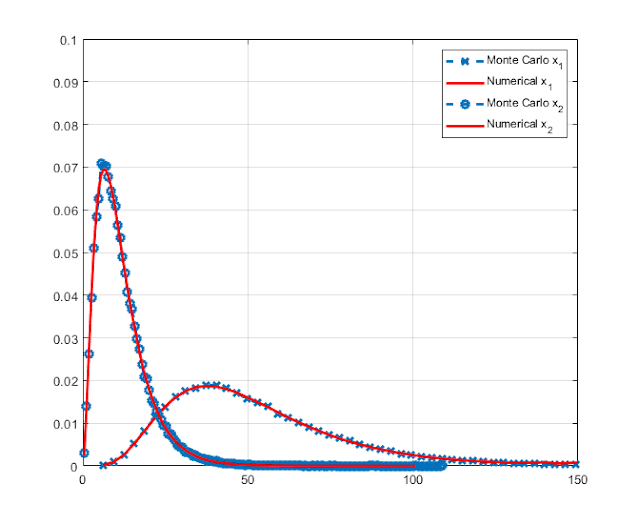
\includegraphics[width=0.9\textwidth,keepaspectratio]{015_004_1.png}
\end{figure}

- ARK

\subsection{Version History}
\begin{enumerate}
	\item \emph{First published: 9th Jul. 2022 on aravindhk-math.blogspot.com}
	\item \emph{Edited: 16th Dec. 2023 -- converted theorem and proof images to \LaTeX}
\end{enumerate}




% ================================================================================
% Bibliography
% ================================================================================
\bibliographystyle{unsrt}
\bibliography{IEEEabrv,references}
%%%%%%%%%%%%%%%%%%%%%%%%%%%%%%%%%%%%%%%%%%%%%%%%%%%%%%%%%%%%%%%%%%%%%%%%%%%%%%%%
\end{document}
